%%%%%%%%%%%%%%%%%%%%%%%%%%%%%%%%%%%%%%%%%%%%%%%%%
% Chapter: API Server
%%%%%%%%%%%%%%%%%%%%%%%%%%%%%%%%%%%%%%%%%%%%%%%%%
\chapter{Server-Specific Interfaces}
\label{chap:api_server}

The \ac{RM} daemon that hosts the \ac{PMIx} server library interacts with that library in two distinct manners. First, \ac{PMIx} provides a set of \acp{API} by which the host can request specific services from its library. This includes generating regular expressions, registering information to be passed to client processes, and requesting information on behalf of a remote process. Note that the host always has access to all \ac{PMIx} client \acp{API} - the functions listed below are in addition to those available to a \ac{PMIx} client.

Second, the host can provide a set of callback functions by which the \ac{PMIx} server library can pass requests upward for servicing by the host. These include notifications of client connection and finalize, as well as requests by clients for information and/or services that the \ac{PMIx} server library does not itself provide.

%%%%%%%%%%%
\section{Server Support Functions}

The following \acp{API} allow the \ac{RM} daemon that hosts the \ac{PMIx} server library to request specific services from the \ac{PMIx} library.

%%%%%%%%%%%
\subsection{\code{PMIx_generate_regex}}
\declareapi{PMIx_generate_regex}

%%%%
\summary

Generate a regular expression representation of the input string.

%%%%
\format

\versionMarker{1.0}
\cspecificstart
\begin{codepar}
pmix_status_t
PMIx_generate_regex(const char *input, char **regex)
\end{codepar}
\cspecificend

\begin{arglist}
\argin{input}{String to process (string)}
\argout{regex}{Regular expression representation of \refarg{input} (string)}
\end{arglist}

Returns \refconst{PMIX_SUCCESS} or a negative value corresponding to a PMIx error constant.

%%%%
\descr

Given a comma-separated list of \refarg{input} values, generate a regular expression that can be passed down to the \ac{PMIx} client for parsing.
The caller is responsible for free'ing the resulting string.

If values have leading zero's, then that is preserved, as are prefix and suffix strings. For example, an input string of ``\code{odin009.org,odin010.org,odin011.org,odin012.org,odin[102-107].org}'' will return a regular expression of ``\code{pmix:odin[009-012,102-107].org}''

\adviceuserstart
The returned regular expression will have a ``\code{pmix:}'' at the beginning of the string. This informs the \ac{PMIx} parser that the string was produced using the \ac{PRI}'s regular expression generator, and thus that same plugin should be used for parsing the string
\adviceuserend


%%%%%%%%%%%
\subsection{\code{PMIx_generate_ppn}}
\declareapi{PMIx_generate_ppn}

%%%%
\summary

Generate a regular expression representation of the input string.

%%%%
\format

\versionMarker{1.0}
\cspecificstart
\begin{codepar}
pmix_status_t PMIx_generate_ppn(const char *input, char **ppn)
\end{codepar}
\cspecificend

\begin{arglist}
\argin{input}{String to process (string)}
\argout{regex}{Regular expression representation of \refarg{input} (string)}
\end{arglist}

Returns \refconst{PMIX_SUCCESS} or a negative value corresponding to a PMIx error constant.

%%%%
\descr

The input is expected to consist of a semicolon-separated list of ranges representing the ranks of processes on each node of the job. Thus, an input of "1-4;2-5;8,10,11,12;6,7,9" would generate a regex of "pmix:2x(3);8,10-12;6-7,9"

\adviceuserstart
The returned regular expression will have a ``pmix:'' at the beginning of the string. This informs the \ac{PMIx} parser that the string was produced using the \ac{PRI}'s regular expression generator, and thus that same plugin should be used for parsing the string
\adviceuserend

%%%%%%%%%%%
\subsection{\code{PMIx_server_register_nspace}}
\declareapi{PMIx_server_register_nspace}

%%%%
\summary

Setup the data about a particular namespace.

%%%%
\format

\versionMarker{1.0}
\cspecificstart
\begin{codepar}
pmix_status_t
PMIx_server_register_nspace(const pmix_nspace_t nspace,
                        int nlocalprocs,
                        pmix_info_t info[], size_t ninfo,
                        pmix_op_cbfunc_t cbfunc, void *cbdata)
\end{codepar}
\cspecificend

\begin{arglist}
\argin{nspace}{namespace (string)}
\argin{nlocalprocs}{number of local processes (integer)}
\argin{info}{Array of info structures (array of handles)}
\argin{ninfo}{Number of elements in the \refarg{info} array (integer)}
\argin{cbfunc}{Callback function \refapi{pmix_op_cbfunc_t} (function reference)}
\argin{cbdata}{Data to be passed to the callback function (memory reference)}
\end{arglist}

Returns one of the following:

\begin{itemize}
    \item \refconst{PMIX_SUCCESS}, indicating that the request is being processed by the host environment - result will be returned in the provided \refarg{cbfunc}. Note that the library \emph{must not} invoke the callback function prior to returning from the \ac{API}.
    \item \refconst{PMIX_OPERATION_SUCCEEDED}, indicating that the request was immediately processed and returned \textit{success} - the \refarg{cbfunc} will \textit{not} be called
    \item a PMIx error constant indicating either an error in the input or that the request was immediately processed and failed - the \refarg{cbfunc} will \textit{not} be called
\end{itemize}

\reqattrstart
The following attributes are \textit{required} to be supported by all \ac{PMIx} libraries:

\pastePRIAttributeItem{PMIX_REGISTER_NODATA}

Host environments are \textit{required} to provide the following attributes:

\begin{itemize}
    \item for the session containing the given namespace:
        \begin{itemize}
            \item \pastePRRTEAttributeItem{PMIX_UNIV_SIZE}
        \end{itemize}
    \item for the given namespace:
        \begin{itemize}
            \item \pastePRRTEAttributeItem{PMIX_JOBID}
            \item \pastePRRTEAttributeItem{PMIX_JOB_SIZE}
            \item \pastePRRTEAttributeItem{PMIX_MAX_PROCS}
            \item \pastePRRTEAttributeItem{PMIX_NODE_MAP}
            \item \pastePRRTEAttributeItem{PMIX_PROC_MAP}
        \end{itemize}
    \item for its own node:
        \begin{itemize}
            \item \pastePRRTEAttributeItem{PMIX_LOCAL_SIZE}
            \item \pastePRRTEAttributeItem{PMIX_LOCAL_PEERS}
            \item \pastePRRTEAttributeItem{PMIX_LOCAL_CPUSETS}
        \end{itemize}
    \item for each process in the given namespace:
        \begin{itemize}
            \item \pastePRRTEAttributeItem{PMIX_RANK}
            \item \pastePRRTEAttributeItem{PMIX_LOCAL_RANK}
            \item \pastePRRTEAttributeItem{PMIX_NODE_RANK}
            \item \pastePRRTEAttributeItem{PMIX_NODEID}
        \end{itemize}
\end{itemize}

If more than one application is included in the namespace, then the host environment is also \textit{required} to provide the following attributes:

\begin{itemize}
    \item for each application:
        \begin{itemize}
            \item \pastePRRTEAttributeItem{PMIX_APPNUM}
            \item \pastePRRTEAttributeItem{PMIX_APPLDR}
            \item \pastePRRTEAttributeItem{PMIX_APP_SIZE}
        \end{itemize}
    \item for each process:
        \begin{itemize}
            \item \pastePRRTEAttributeItem{PMIX_APP_RANK}
            \item \pastePRRTEAttributeItem{PMIX_APPNUM}
        \end{itemize}
\end{itemize}

\reqattrend


\optattrstart

The following attributes \textit{may} be provided by host environments:

\begin{itemize}
    \item for the session containing the given namespace:
        \begin{itemize}
            \item \pastePRRTEAttributeItem{PMIX_SESSION_ID}
        \end{itemize}
    \item for the given namespace:
        \begin{itemize}
            \item \pastePRRTEAttributeItem{PMIX_SERVER_NSPACE}
            \item \pastePRRTEAttributeItem{PMIX_SERVER_RANK}
            \item \pastePRRTEAttributeItem{PMIX_NPROC_OFFSET}
            \item \pastePRRTEAttributeItem{PMIX_ALLOCATED_NODELIST}
            \item \pastePRRTEAttributeItem{PMIX_JOB_NUM_APPS}
            \item \pastePRRTEAttributeItem{PMIX_MAPBY}
            \item \pastePRRTEAttributeItem{PMIX_RANKBY}
            \item \pastePRRTEAttributeItem{PMIX_BINDTO}
        \end{itemize}
    \item for its own node:
        \begin{itemize}
            \item \pastePRRTEAttributeItem{PMIX_AVAIL_PHYS_MEMORY}
            \item \pastePRRTEAttributeItem{PMIX_HWLOC_XML_V1}
            \item \pastePRRTEAttributeItem{PMIX_HWLOC_XML_V2}
            \item \pastePRRTEAttributeItem{PMIX_LOCALLDR}
            \item \pastePRRTEAttributeItem{PMIX_NODE_SIZE}
            \item \pastePRRTEAttributeItem{PMIX_LOCAL_PROCS}
        \end{itemize}
    \item for each process in the given namespace:
        \begin{itemize}
            \item \pastePRRTEAttributeItem{PMIX_PROCID}
            \item \pastePRRTEAttributeItem{PMIX_GLOBAL_RANK}
            \item \pastePRRTEAttributeItem{PMIX_HOSTNAME}
        \end{itemize}
\end{itemize}

Attributes not directly provided by the host environment \textit{may} be derived by the \ac{PMIx} server library from other required information and included in the data made available to the server library's clients.

\optattrend

%%%%
\descr

Pass job-related information to the \ac{PMIx} server library for distribution to local client processes.

\advicermstart
Host environments are \textit{required} to execute this operation prior to starting any local application process within the given namespace.

The \ac{PMIx} server must register \emph{all} namespaces that will participate in collective operations with local processes.
This means that the server must register a namespace even if it will not host any local processes from within that namespace \emph{if} any local process of another namespace might at some point perform an operation involving one or more processes from the new namespace.
This is necessary so that the collective operation can identify the participants and know when it is locally complete.

The caller must also provide the number of local processes that will be launched within this namespace.
This is required for the \ac{PMIx} server library to correctly handle collectives as a collective operation call can occur before all the local processes have been started.
\advicermend

\adviceuserstart
The number of local processes for any given namespace is generally fixed at the time of application launch. Calls to \refapi{PMIx_Spawn} result in processes launched in their own namespace, not that of their parent. However, it is possible for processes to \textit{migrate} to another node via a call to \refapi{PMIx_Job_control_nb}, thus resulting in a change to the number of local processes on both the initial node and the node to which the process moved. It is therefore \textit{critical} that applications not migrate processes without first ensuring that \ac{PMIx}-based collective operations are not in progress, and that no such operations be initiated until process migration has completed.
\adviceuserend


%%%%%%%%%%%
\subsubsection{Assembling the registration information}
\label{chap:api_server:assemble}

The following description is not intended to represent the actual layout of information in a given \ac{PMIx} library. Instead, it is describes how information provided in the \refarg{info} parameter of the \refapi{PMIx_server_register_nspace} shall be organized for proper processing by a \ac{PMIx} server library. The ordering of the various information elements is arbitrary - they are presented in a top-down hierarchical form solely for clarity in reading.

\advicermstart
Creating the \refarg{info} array of data requires knowing in advance the number of elements required for the array. This can be difficult to compute and somewhat fragile in practice. One method for resolving the problem is to create a linked list of objects, each containing a single \refstruct{pmix_info_t} structure. Allocation and manipulation of the list can then be accomplished using existing standard methods. Upon completion, the final \refarg{info} array can be allocated based on the number of elements on the list, and then the values in the list object \refstruct{pmix_info_t} structures transferred to the corresponding array element utilizing the \refmacro{PMIX_INFO_XFER} macro.
\advicermend

\label{cptr:api_server:noderegex}A common building block used in several areas is the construction of a regular expression identifying the nodes involved in that area - e.g., the nodes in a \refterm{session} or \refterm{job}. \ac{PMIx} provides several tools to facilitate this operation, beginning by constructing an argv-like array of node names. This array is then passed to the \refapi{PMIx_generate_regex} function to create a regular expression parseable by the \ac{PMIx} server library, as shown below:

\cspecificstart
\begin{codepar}
char **nodes = NULL;
char *nodelist;
char *regex;
size_t n;
pmix_status_t rc;
pmix_info_t info;

/* loop over an array of nodes, adding each
 * name to the array */
for (n=0; n < num_nodes; n++) {
    /* filter the nodes to ignore those not included
     * in the target range (session, job, etc.). In
     * this example, all nodes are accepted */
    PMIX_ARGV_APPEND(&nodes, node[n]->name);
}

/* join into a comma-delimited string */
nodelist = PMIX_ARGV_JOIN(nodes, ',');

/* release the array */
PMIX_ARGV_FREE(nodes);

/* generate regex */
rc = PMIx_generate_regex(nodelist, &regex);

/* release list */
free(nodelist);

/* pass the regex as the value to the PMIX_NODE_MAP key */
PMIX_INFO_LOAD(&info, PMIX_NODE_MAP, regex, PMIX_STRING);
/* release the regex */
free(regex);

\end{codepar}
\cspecificend

Changing the filter criteria allows the construction of node maps for any level of information.

\label{cptr:api_server:ppnregex}A similar method is used to construct the map of processes on each node from the namespace being registered. This may be done for each information level of interest (e.g., to identify the process map for the entire \refterm{job} or for each \refterm{application} in the job) by changing the search criteria. An example is shown below for the case of creating the process map for a \refterm{job}:

\cspecificstart
\begin{codepar}
char **ndppn;
char rank[30];
char **ppnarray = NULL;
char *ppn;
char *localranks;
char *regex;
size_t n, m;
pmix_status_t rc;
pmix_info_t info;

/* loop over an array of nodes */
for (n=0; n < num_nodes; n++) {
    /* for each node, construct an array of ranks on that node */
    ndppn = NULL;
    for (m=0; m < node[n]->num_procs; m++) {
        /* ignore processes that are not part of the target job */
        if (!PMIX_CHECK_NSPACE(targetjob,node[n]->proc[m].nspace)) {
            continue;
        }
        snprintf(rank, 30, "%d", node[n]->proc[m].rank);
        PMIX_ARGV_APPEND(&ndppn, rank);
    }
    /* convert the array into a comma-delimited string of ranks */
    localranks = PMIX_ARGV_JOIN(ndppn, ',');
    /* release the local array */
    PMIX_ARGV_FREE(ndppn);
    /* add this node's contribution to the overall array */
    PMIX_ARGV_APPEND(&ppnarray, localranks);
    /* release the local list */
    free(localranks);
}

/* join into a semicolon-delimited string */
ppn = PMIX_ARGV_JOIN(ppnarray, ';');

/* release the array */
PMIX_ARGV_FREE(ppnarray);

/* generate ppn regex */
rc = PMIx_generate_ppn(ppn, &regex);

/* release list */
free(ppn);

/* pass the regex as the value to the PMIX_PROC_MAP key */
PMIX_INFO_LOAD(&info, PMIX_PROC_MAP, regex, PMIX_STRING);
/* release the regex */
free(regex);

\end{codepar}
\cspecificend

Note that the \refattr{PMIX_NODE_MAP} and \refattr{PMIX_PROC_MAP} attributes are linked in that the order of entries in the process map must match the ordering of nodes in the node map - i.e., there is no provision in the \ac{PMIx} process map regular expression generator/parser pair supporting an out-of-order node or a node that has no corresponding process map entry (e.g., a node with no processes on it). Armed with these tools, the registration \refarg{info} array can be constructed as follows:

\begin{itemize}
\item Session-level information includes all session-specific values. In many cases, only two values (\refattr{PMIX_SESSION_ID} and \refattr{PMIX_UNIV_SIZE}) are included in the registration array. Since both of these values are session-specific, they can be specified independently - i.e., in their own \refstruct{pmix_info_t} elements of the \refarg{info} array. Alternatively, they can be provided as a \refstruct{pmix_data_array_t} array of \refstruct{pmix_info_t} using the \refattr{PMIX_SESSION_INFO_ARRAY} attribute and identifed by including the \refattr{PMIX_SESSION_ID} attribute in the array - this is \emph{required} in cases where non-specific attributes (e.g., \refattr{PMIX_NUM_NODES} or \refattr{PMIX_NODE_MAP}) are passed to describe aspects of the session. Note that the node map can include nodes not used by the job being registered as no corresponding process map is specified.

The \refarg{info} array at this point might look like (where the labels identify the corresponding attribute - e.g., ``Session ID'' corresponds to the \refattr{PMIX_SESSION_ID} attribute):

\begingroup
\begin{figure*}[ht!]
  \begin{center}
    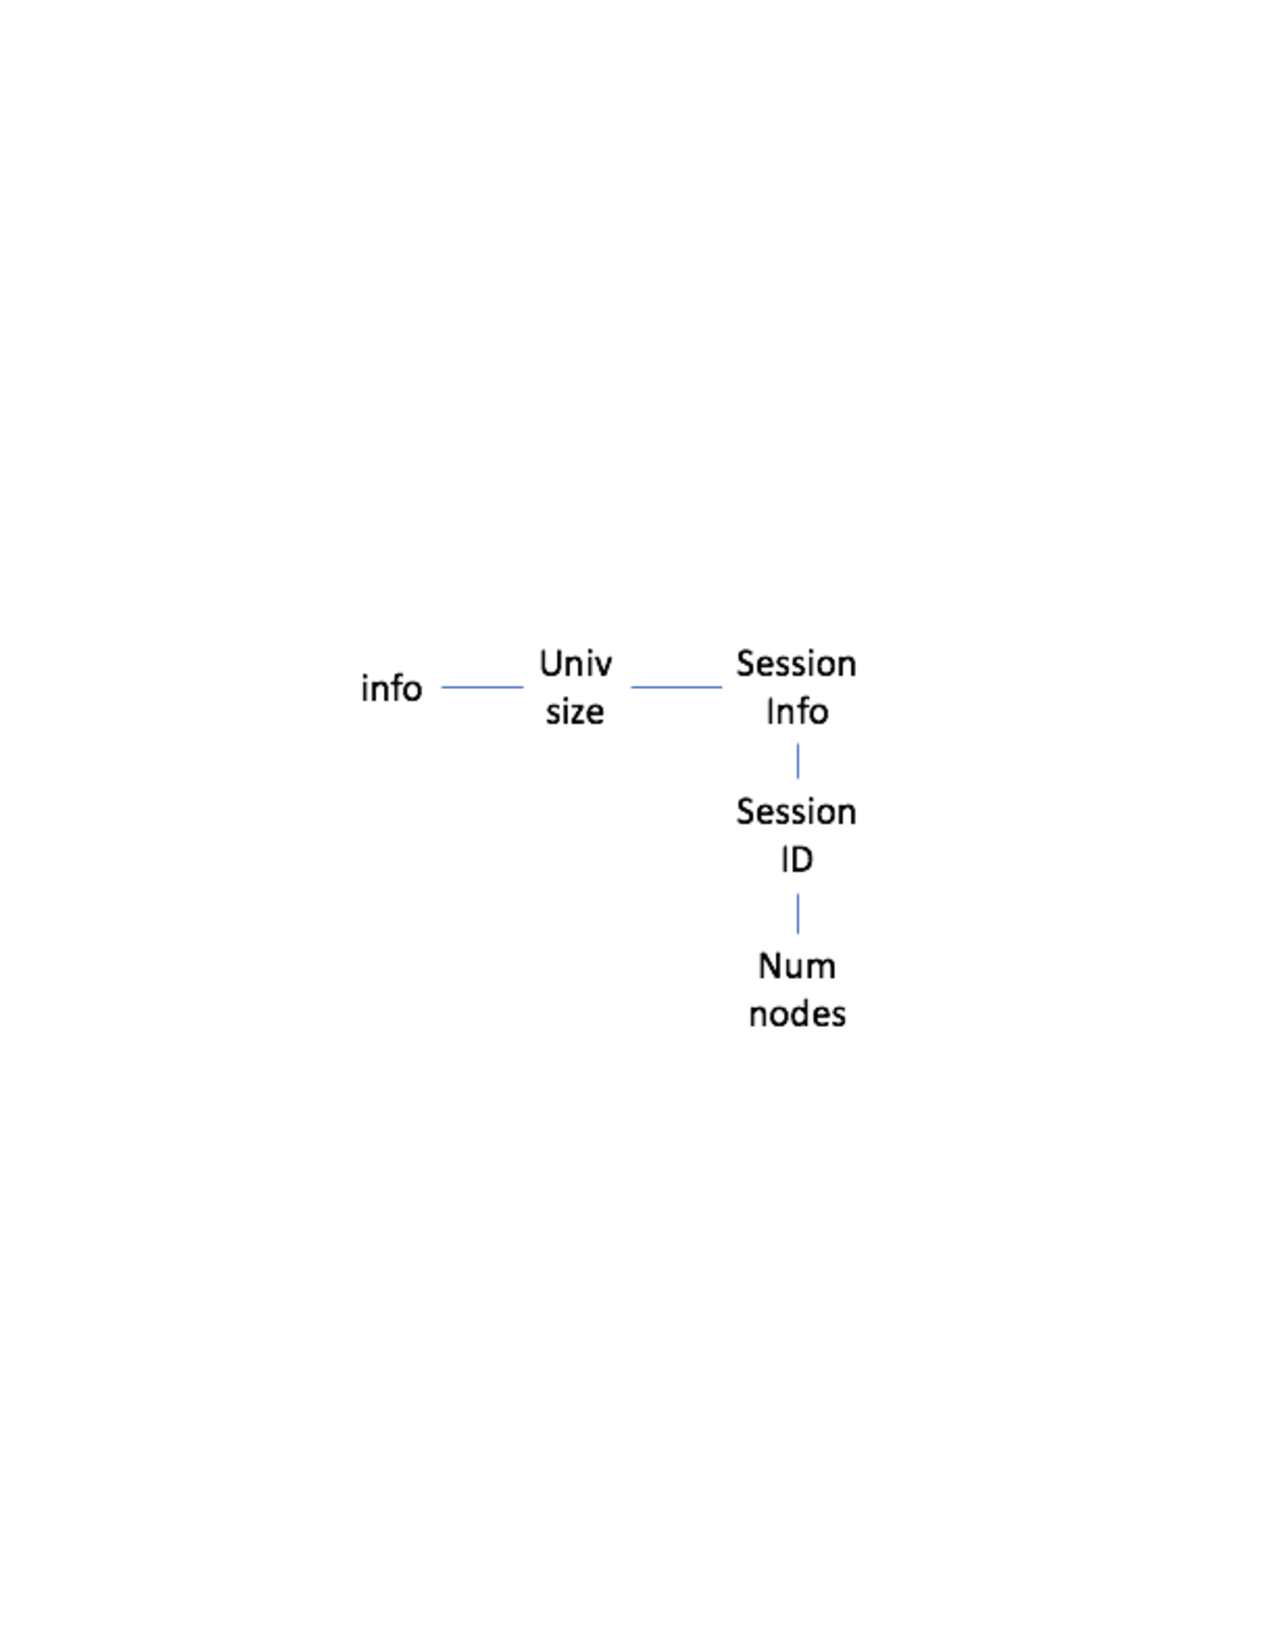
\includegraphics[clip,width=0.3\textwidth]{figs/sessioninfo.pdf}
  \end{center}
  \caption{Session-level information elements}
  \label{fig:sessioninfo}
\end{figure*}
\endgroup


\item Job-level information includes all job-specific values such as \refattr{PMIX_JOB_SIZE}, \refattr{PMIX_JOB_NUM_APPS}, and \refattr{PMIX_JOBID}. Since each invocation of \refapi{PMIx_server_register_nspace} describes a single \refterm{job}, job-specific values can be specified independently - i.e., in their own \refstruct{pmix_info_t} elements of the \refarg{info} array. Alternatively, they can be provided as a \refstruct{pmix_data_array_t} array of \refstruct{pmix_info_t} identified by the \refattr{PMIX_JOB_INFO_ARRAY} attribute - this is \emph{required} in cases where non-specific attributes (e.g., \refattr{PMIX_NODE_MAP}) are passed to describe aspects of the job. Note that since the invocation only involves a single namespace, there is no need to include the \refattr{PMIX_NSPACE} attribute in the array.

Upon conclusion of this step, the \refarg{info} array might look like:

\begingroup
\begin{figure*}[ht!]
  \begin{center}
    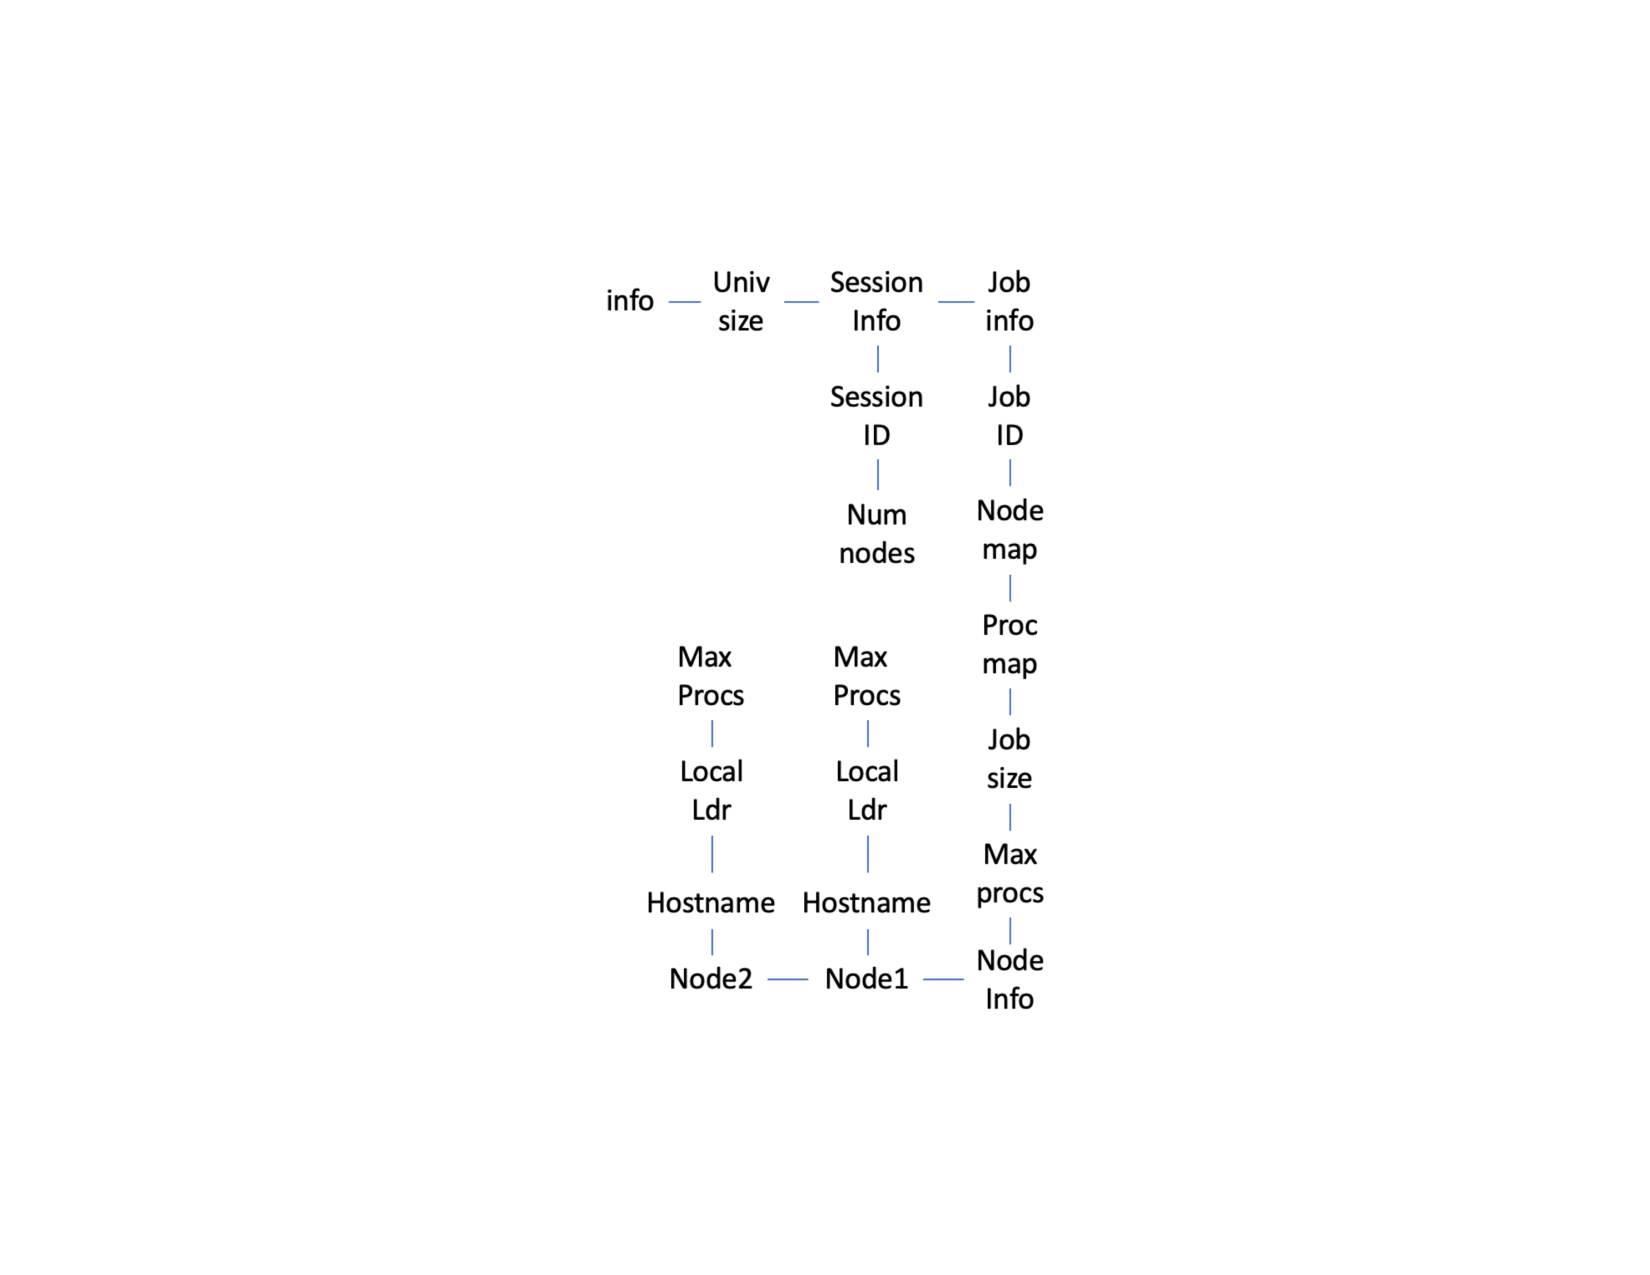
\includegraphics[clip,width=0.4\textwidth]{figs/jobinfo.pdf}
  \end{center}
  \caption{Job-level information elements}
  \label{fig:jobinfo}
\end{figure*}
\endgroup

Note that in this example, \refattr{PMIX_NUM_NODES} is not required as that information is contained in the \refattr{PMIX_NODE_MAP} attribute. Similarly, \refattr{PMIX_JOB_SIZE} is not technically required as that information is contained in the \refattr{PMIX_PROC_MAP} when combined with the corresponding node map - however, there is no issue with including the job size as a separate entry.

\item Application-level information includes all application-specific values such as \refattr{PMIX_APP_SIZE} and \refattr{PMIX_APPLDR}. If the \refterm{job} contains only a single \refterm{application}, then the application-specific values can be specified independently - i.e., in their own \refstruct{pmix_info_t} elements of the \refarg{info} array - or as a \refstruct{pmix_data_array_t} array of \refstruct{pmix_info_t} using the \refattr{PMIX_APP_INFO_ARRAY} attribute and identifed by including the \refattr{PMIX_APPNUM} attribute in the array. Use of the array format is  \emph{required} in cases where non-specific attributes (e.g., \refattr{PMIX_NODE_MAP}) are passed to describe aspects of the application.

However, in the case of a job consisting of multiple applications, all application-specific values for each application \emph{must} be provided using the \refattr{PMIX_APP_INFO_ARRAY} format, each identified by its \refattr{PMIX_APPNUM} value.

Upon conclusion of this step, the \refarg{info} array might look like that shown in \ref{fig:appinfo}, assuming there are two applications in the job being registered:

\begingroup
\begin{figure*}[ht!]
  \begin{center}
    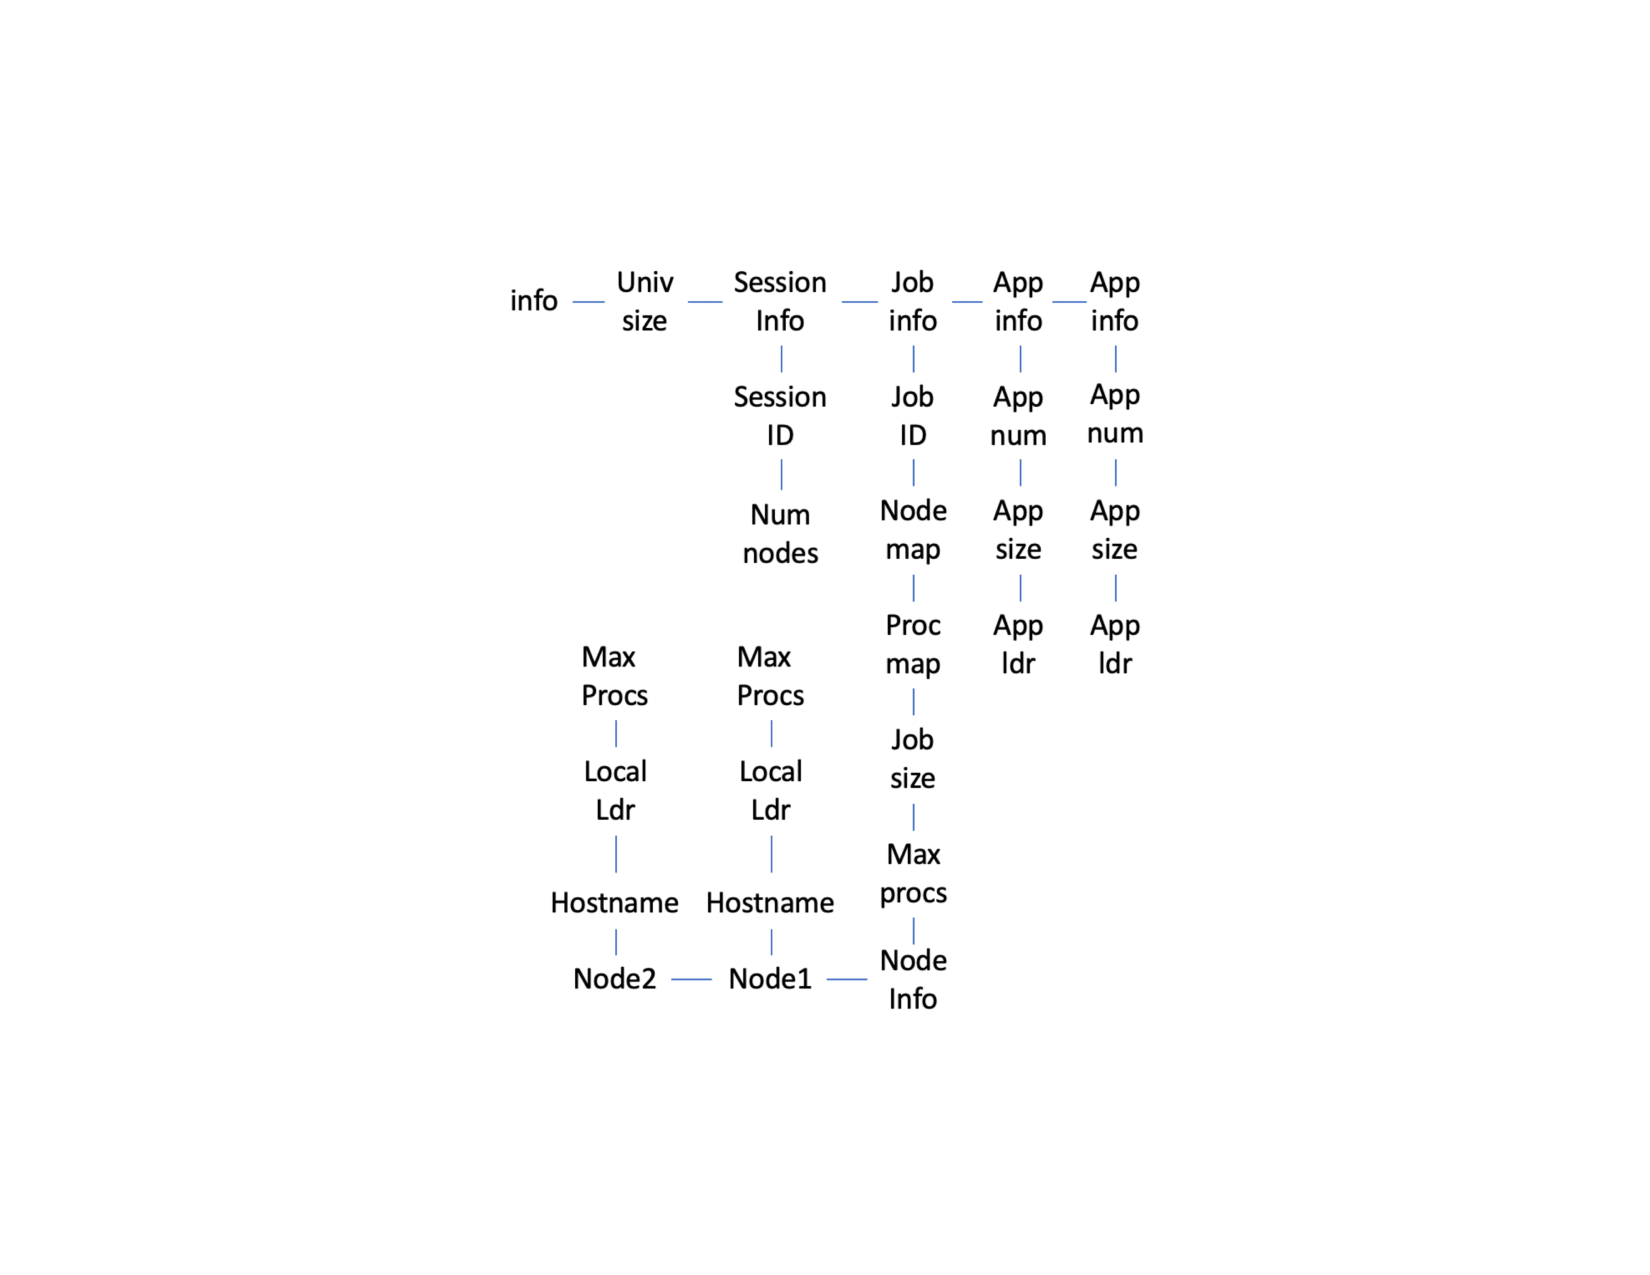
\includegraphics[clip,width=0.5\textwidth]{figs/appinfo.pdf}
  \end{center}
  \caption{Application-level information elements}
  \label{fig:appinfo}
\end{figure*}
\endgroup

\item Process-level information includes an entry for each process in the job being registered, each entry marked with the \refattr{PMIX_PROC_DATA} attribute. The \refterm{rank} of the process \emph{must} be the first entry in the array - this provides efficiency when storing the data. Upon conclusion of this step, the \refarg{info} array might look like the diagram in \ref{fig:procinfo}:

\begingroup
\begin{figure*}[ht!]
  \begin{center}
    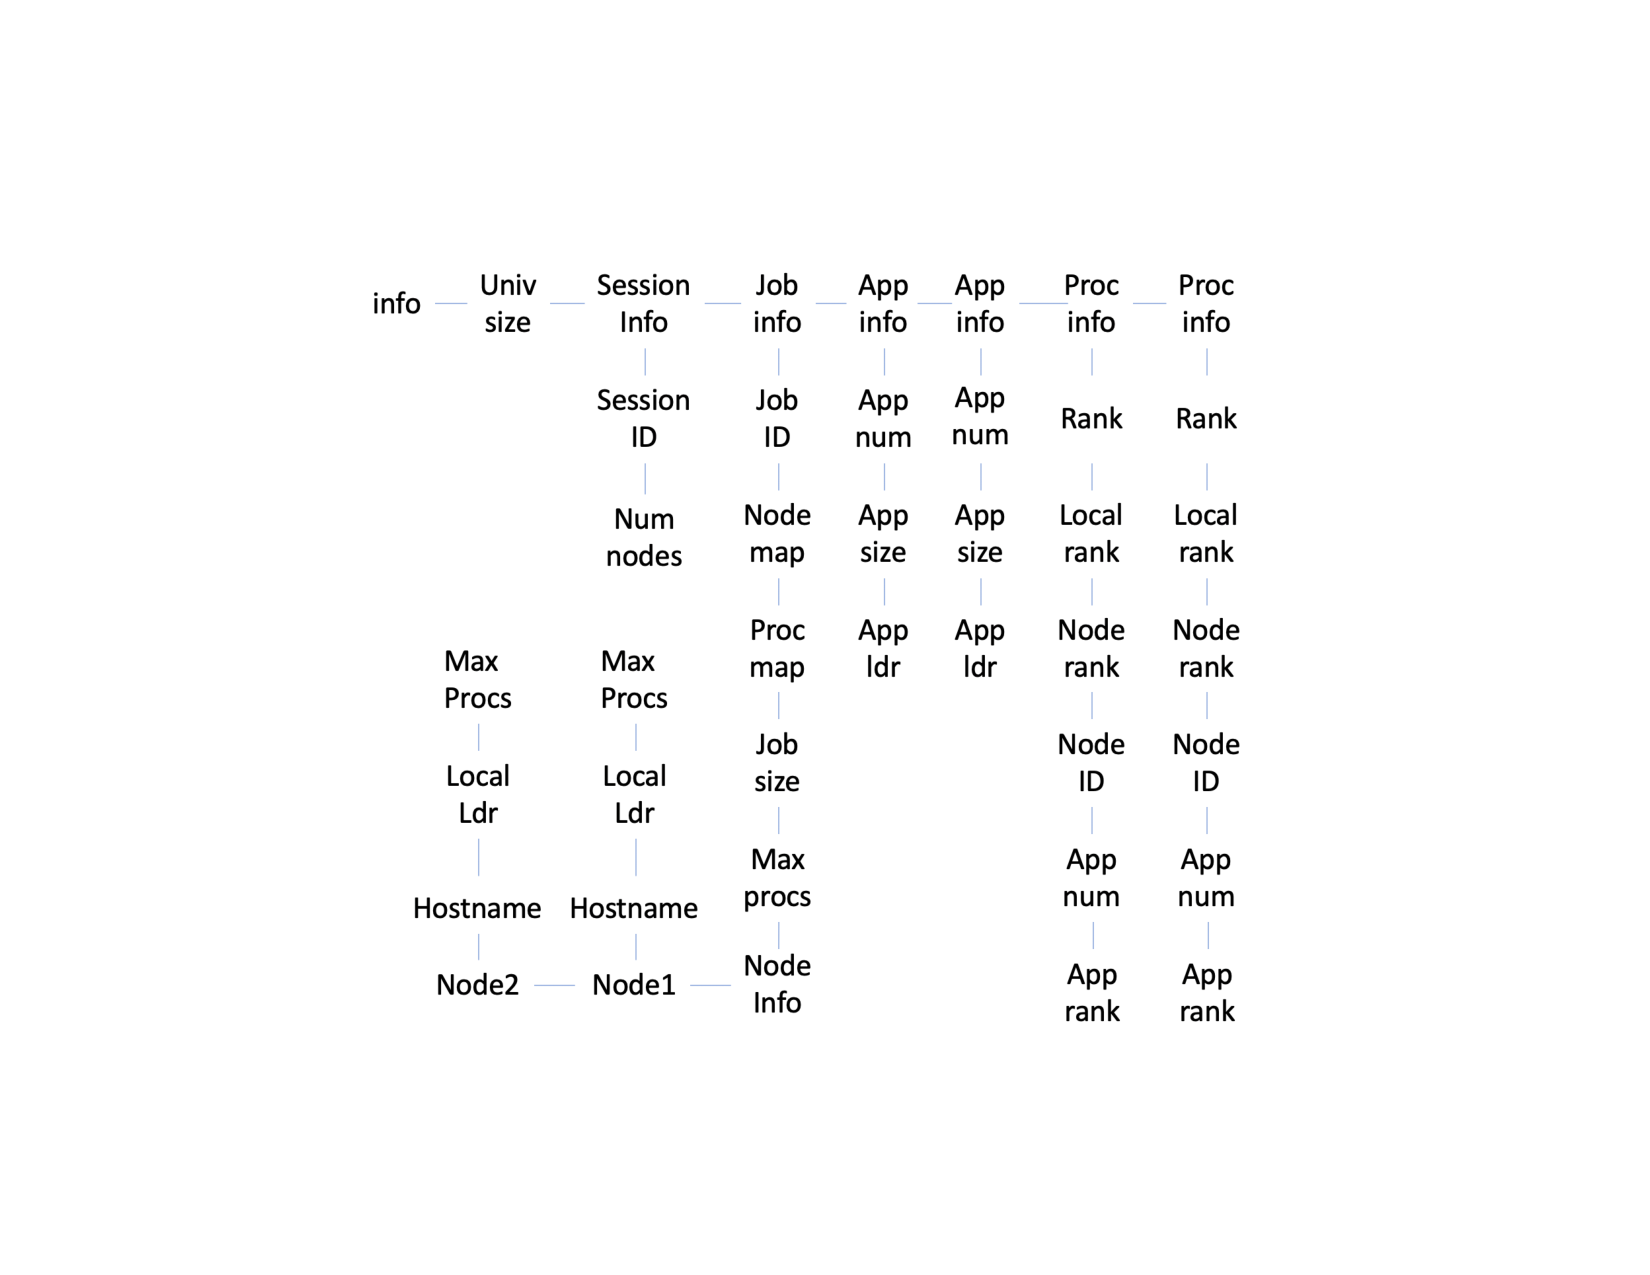
\includegraphics[clip,width=0.5\textwidth]{figs/procinfo.pdf}
  \end{center}
  \caption{Process-level information elements}
  \label{fig:procinfo}
\end{figure*}
\endgroup

\item Node-level information only includes values describing the local node - i.e., it does not include information about other nodes in the job or session. In many cases, the values included in this level are unique to it and can be specified independently - i.e., in their own \refstruct{pmix_info_t} elements of the \refarg{info} array. Alternatively, they can be provided as a \refstruct{pmix_data_array_t} array of \refstruct{pmix_info_t} using the \refattr{PMIX_NODE_INFO_ARRAY} attribute - this is \emph{required} in cases where non-specific attributes are passed to describe aspects of the node.

The node-level information requires two elements that must be constructed in a manner similar to that used for the node map. The \refattr{PMIX_LOCAL_PEERS} value is computed based on the processes on the local node, filtered to select those from the job being registered, as shown below using the tools provided by \ac{PMIx}:

\cspecificstart
\begin{codepar}
char **ndppn = NULL;
char rank[30];
char *localranks;
size_t m;
pmix_info_t info;

for (m=0; m < mynode->num_procs; m++) {
    /* ignore processes that are not part of the target job */
    if (!PMIX_CHECK_NSPACE(targetjob,mynode->proc[m].nspace)) {
        continue;
    }
    snprintf(rank, 30, "%d", mynode->proc[m].rank);
    PMIX_ARGV_APPEND(&ndppn, rank);
}
/* convert the array into a comma-delimited string of ranks */
localranks = PMIX_ARGV_JOIN(ndppn, ',');
/* release the local array */
PMIX_ARGV_FREE(ndppn);

/* pass the string as the value to the PMIX_LOCAL_PEERS key */
PMIX_INFO_LOAD(&info, PMIX_LOCAL_PEERS, localranks, PMIX_STRING);
/* release the list */
free(localranks);

\end{codepar}
\cspecificend

The \refattr{PMIX_LOCAL_CPUSETS} value is constructed in a similar manner. In the provided example, it is assumed that the \ac{HWLOC} cpuset representation (a comma-delimited string of processor IDs) of the processors assigned to each process has previously been generated and stored on the process description. Thus, the value can be constructed as shown below:

\cspecificstart
\begin{codepar}
char **ndcpus = NULL;
char *localcpus;
size_t m;
pmix_info_t info;

for (m=0; m < mynode->num_procs; m++) {
    /* ignore processes that are not part of the target job */
    if (!PMIX_CHECK_NSPACE(targetjob,mynode->proc[m].nspace)) {
        continue;
    }
    PMIX_ARGV_APPEND(&ndcpus, mynode->proc[m].cpuset);
}
/* convert the array into a colon-delimited string */
localcpus = PMIX_ARGV_JOIN(ndcpus, ':');
/* release the local array */
PMIX_ARGV_FREE(ndcpus);

/* pass the string as the value to the PMIX_LOCAL_CPUSETS key */
PMIX_INFO_LOAD(&info, PMIX_LOCAL_CPUSETS, localcpus, PMIX_STRING);
/* release the list */
free(localcpus);

\end{codepar}
\cspecificend

Note that for efficiency, these two values can be computed at the same time.

\end{itemize}

The final \refarg{info} array might therefore look like the diagram in \ref{fig:nodeinfo}:

\begingroup
\begin{figure*}[ht!]
  \begin{center}
    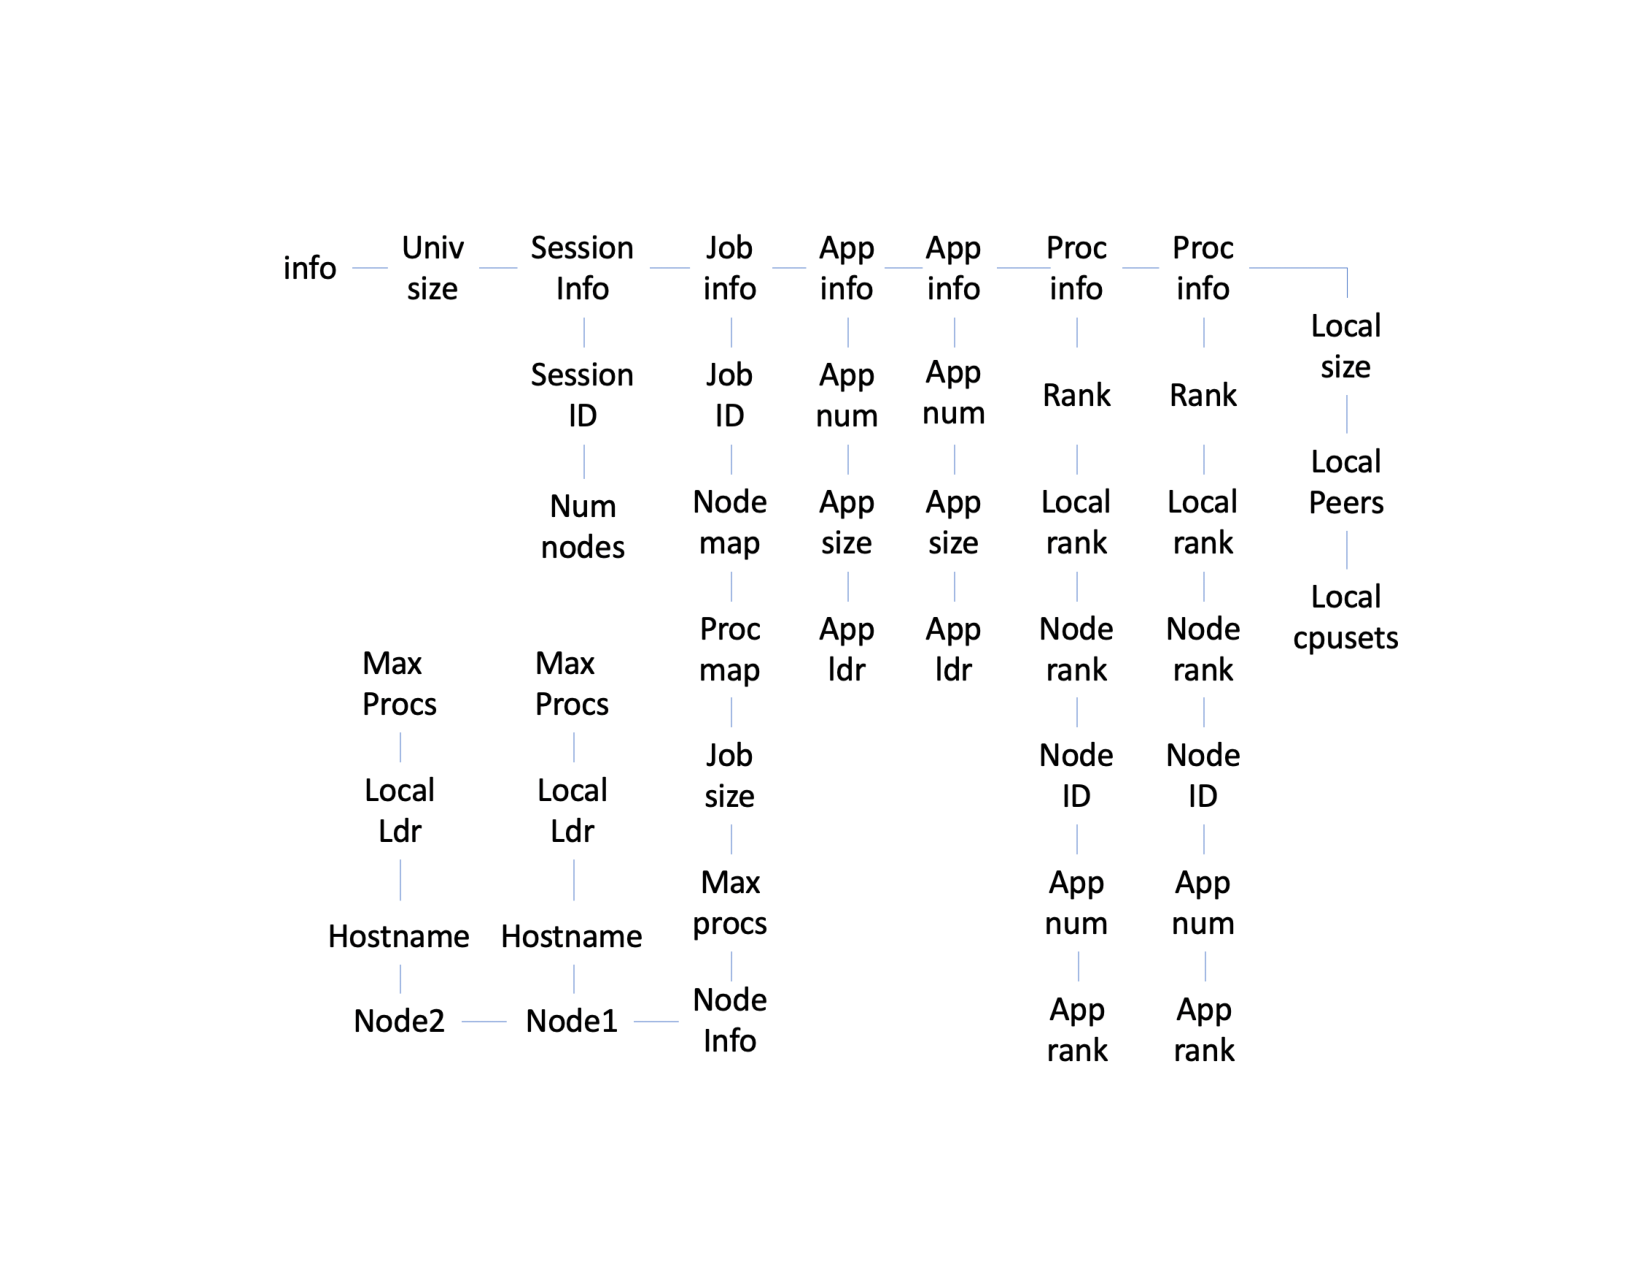
\includegraphics[clip,width=0.8\textwidth]{figs/nodeinfo.pdf}
  \end{center}
  \caption{Final information array}
  \label{fig:nodeinfo}
\end{figure*}
\endgroup


%%%%%%%%%%%
\subsection{\code{PMIx_server_deregister_nspace}}
\declareapi{PMIx_server_deregister_nspace}

%%%%
\summary

Deregister a namespace.

%%%%
\format

\versionMarker{1.0}
\cspecificstart
\begin{codepar}
void PMIx_server_deregister_nspace(const pmix_nspace_t nspace,
                        pmix_op_cbfunc_t cbfunc, void *cbdata)
\end{codepar}
\cspecificend

\begin{arglist}
\argin{nspace}{Namespace (string)}
\argin{cbfunc}{Callback function \refapi{pmix_op_cbfunc_t} (function reference)}
\argin{cbdata}{Data to be passed to the callback function (memory reference)}
\end{arglist}

%%%%
\descr

Deregister the specified \refarg{nspace} and purge all objects relating to it, including any client information from that namespace.
This is intended to support persistent \ac{PMIx} servers by providing an opportunity for the host \ac{RM} to tell the \ac{PMIx} server library to release all memory for a completed job. Note that the library \emph{must not} invoke the callback function prior to returning from the \ac{API}.


%%%%%%%%%%%
\subsection{\code{PMIx_server_register_client}}
\declareapi{PMIx_server_register_client}

%%%%
\summary

Register a client process with the PMIx server library.

%%%%
\format

\versionMarker{1.0}
\cspecificstart
\begin{codepar}
pmix_status_t
PMIx_server_register_client(const pmix_proc_t *proc,
                        uid_t uid, gid_t gid,
                        void *server_object,
                        pmix_op_cbfunc_t cbfunc, void *cbdata)
\end{codepar}
\cspecificend

\begin{arglist}
\argin{proc}{\refstruct{pmix_proc_t} structure (handle)}
\argin{uid}{user id (integer)}
\argin{gid}{group id (integer)}
\argin{server_object}{(memory reference)}
\argin{cbfunc}{Callback function \refapi{pmix_op_cbfunc_t} (function reference)}
\argin{cbdata}{Data to be passed to the callback function (memory reference)}
\end{arglist}

Returns one of the following:

\begin{itemize}
    \item \refconst{PMIX_SUCCESS}, indicating that the request is being processed by the host environment - result will be returned in the provided \refarg{cbfunc}. Note that the library \emph{must not} invoke the callback function prior to returning from the \ac{API}.
    \item \refconst{PMIX_OPERATION_SUCCEEDED}, indicating that the request was immediately processed and returned \textit{success} - the \refarg{cbfunc} will \textit{not} be called
    \item a PMIx error constant indicating either an error in the input or that the request was immediately processed and failed - the \refarg{cbfunc} will \textit{not} be called
\end{itemize}


%%%%
\descr

Register a client process with the PMIx server library.

The host server can also, if it desires, provide an object it wishes to be returned when a server function is called that relates to a specific process.
For example, the host server may have an object that tracks the specific client.
Passing the object to the library allows the library to provide that object to the host server during subsequent calls related to that client, such as a \refapi{pmix_server_client_connected_fn_t} function.  This allows the host server to access the object without performing a lookup based on the client's namespace and rank.

\advicermstart
Host environments are \textit{required} to execute this operation prior to starting the client process.
The expected user ID and group ID of the child process allows the server library to properly authenticate clients as they connect by requiring the two values to match. Accordingly, the detected user and group ID's of the connecting process are not included in the \refapi{pmix_server_client_connected_fn_t} server module function.
\advicermend

\adviceimplstart
For security purposes, the \ac{PMIx} server library should check the user and group ID's of a connecting process against those provided for the declared client process identifier via the \refapi{PMIx_server_register_client} prior to completing the connection.
\adviceimplend

%%%%%%%%%%%
\subsection{\code{PMIx_server_deregister_client}}
\declareapi{PMIx_server_deregister_client}

%%%%
\summary

Deregister a client and purge all data relating to it.

%%%%
\format

\versionMarker{1.0}
\cspecificstart
\begin{codepar}
void
PMIx_server_deregister_client(const pmix_proc_t *proc,
                        pmix_op_cbfunc_t cbfunc, void *cbdata)
\end{codepar}
\cspecificend

\begin{arglist}
\argin{proc}{\refstruct{pmix_proc_t} structure (handle)}
\argin{cbfunc}{Callback function \refapi{pmix_op_cbfunc_t} (function reference)}
\argin{cbdata}{Data to be passed to the callback function (memory reference)}
\end{arglist}


%%%%
\descr

The \refapi{PMIx_server_deregister_nspace} \ac{API} will delete all client information for that namespace. The \ac{PMIx} server library will automatically perform that operation upon disconnect of all local clients.
This \ac{API} is therefore intended primarily for use in exception cases, but can be called in non-exception cases if desired. Note that the library \emph{must not} invoke the callback function prior to returning from the \ac{API}.


%%%%%%%%%%%
\subsection{\code{PMIx_server_setup_fork}}
\declareapi{PMIx_server_setup_fork}

%%%%
\summary

Setup the environment of a child process to be forked by the host.

%%%%
\format

\versionMarker{1.0}
\cspecificstart
\begin{codepar}
pmix_status_t
PMIx_server_setup_fork(const pmix_proc_t *proc,
                        char ***env)
\end{codepar}
\cspecificend

\begin{arglist}
\argin{proc}{\refstruct{pmix_proc_t} structure (handle)}
\argin{env}{Environment array (array of strings)}
\end{arglist}

Returns \refconst{PMIX_SUCCESS} or a negative value corresponding to a PMIx error constant.

%%%%
\descr

Setup the environment of a child process to be forked by the host so it can correctly interact with the PMIx server.

\advicermstart
Host environments are \textit{required} to execute this operation prior to starting the client process.
\advicermend

The \ac{PMIx} client needs some setup information so it can properly connect back to the server.
This function will set appropriate environmental variables for this purpose, and will also provide any environmental variables that were specified in the launch command (e.g., via \refapi{PMIx_Spawn}) plus other values (e.g., variables required to properly initialize the client's fabric library).


%%%%%%%%%%%
\subsection{\code{PMIx_server_dmodex_request}}
\declareapi{PMIx_server_dmodex_request}

%%%%
\summary

Define a function by which the host server can request modex data from the local PMIx server.

%%%%
\format

\versionMarker{1.0}
\cspecificstart
\begin{codepar}
pmix_status_t PMIx_server_dmodex_request(const pmix_proc_t *proc,
                        pmix_dmodex_response_fn_t cbfunc,
                        void *cbdata)
\end{codepar}
\cspecificend

\begin{arglist}
\argin{proc}{\refstruct{pmix_proc_t} structure (handle)}
\argin{cbfunc}{Callback function \refapi{pmix_dmodex_response_fn_t} (function reference)}
\argin{cbdata}{Data to be passed to the callback function (memory reference)}
\end{arglist}

Returns one of the following:

\begin{itemize}
    \item \refconst{PMIX_SUCCESS}, indicating that the request is being processed by the host environment - result will be returned in the provided \refarg{cbfunc}. Note that the library \emph{must not} invoke the callback function prior to returning from the \ac{API}.
    \item a PMIx error constant indicating an error in the input - the \refarg{cbfunc} will \textit{not} be called
\end{itemize}


%%%%
\descr

Define a function by which the host server can request modex data from the local \ac{PMIx} server. Traditional wireup procedures revolve around the per-process posting of data (e.g., location and endpoint information) via the \refapi{PMIx_Put} and \refapi{PMIx_Commit} functions followed by a \refapi{PMIx_Fence} barrier that globally exchanges the posted information. However, the barrier operation represents a signficant time impact at large scale.

\ac{PMIx} supports an alternative wireup method known as \textit{Direct Modex} that replaces the barrier-based exchange of all process-posted information with on-demand fetch of a peer's data. In place of the barrier operation, data posted by each process is cached on the local \ac{PMIx} server. When a process requests the information posted by a particular peer, it first checks the local cache to see if the data is already available. If not, then the request is passed to the local \ac{PMIx} server, which subsequently requests that its \ac{RM} host request the data from the \ac{RM} daemon on the node where the specified peer process is located. Upon receiving the request, the \ac{RM} daemon passes the request into its \ac{PMIx} server library using the \refapi{PMIx_server_dmodex_request} function, receiving the response in the provided \refarg{cbfunc} once the indicated process has posted its information. The \ac{RM} daemon then returns the data to the requesting daemon, who subsequently passes the data to its \ac{PMIx} server library for transfer to the requesting client.

\adviceuserstart
While direct modex allows for faster launch times by eliminating the barrier operation, per-peer retrieval of posted information is less efficient. Optimizations can be implemented - e.g., by returning posted information from all processes on a node upon first request - but in general direct modex remains best suited for sparsely connected applications.
\adviceuserend

%%%%%%%%%%%
\subsection{\code{PMIx_server_setup_application}}
\declareapi{PMIx_server_setup_application}

%%%%
\summary

Provide a function by which the resource manager can request application-specific setup data prior to launch of an application.

%%%%
\format

\versionMarker{2.0}
\cspecificstart
\begin{codepar}
pmix_status_t
PMIx_server_setup_application(const pmix_nspace_t nspace,
                        pmix_info_t info[], size_t ninfo,
                        pmix_setup_application_cbfunc_t cbfunc,
                        void *cbdata)
\end{codepar}
\cspecificend

\begin{arglist}
\argin{nspace}{namespace (string)}
\argin{info}{Array of info structures (array of handles)}
\argin{ninfo}{Number of elements in the \refarg{info} array (integer)}
\argin{cbfunc}{Callback function \refapi{pmix_setup_application_cbfunc_t} (function reference)}
\argin{cbdata}{Data to be passed to the \refarg{cbfunc} callback function (memory reference)}
\end{arglist}

Returns one of the following:

\begin{itemize}
    \item \refconst{PMIX_SUCCESS}, indicating that the request is being processed by the host environment - result will be returned in the provided \refarg{cbfunc}. Note that the library \emph{must not} invoke the callback function prior to returning from the \ac{API}.
    \item a PMIx error constant indicating either an error in the input - the \refarg{cbfunc} will \textit{not} be called
\end{itemize}


\reqattrstart
\ac{PMIx} libraries that support this operation are required to support the following:

\pastePRIAttributeItem{PMIX_SETUP_APP_ENVARS}
\pastePRIAttributeItem{PMIX_SETUP_APP_NONENVARS}
\pastePRIAttributeItem{PMIX_SETUP_APP_ALL}
\pastePRIAttributeItem{PMIX_ALLOC_NETWORK}
\pastePRIAttributeItem{PMIX_ALLOC_NETWORK_ID}
\pastePRIAttributeItem{PMIX_ALLOC_NETWORK_SEC_KEY}
\pastePRIAttributeItem{PMIX_ALLOC_NETWORK_TYPE}
\pastePRIAttributeItem{PMIX_ALLOC_NETWORK_PLANE}
\pastePRIAttributeItem{PMIX_ALLOC_NETWORK_ENDPTS}
\pastePRIAttributeItem{PMIX_ALLOC_NETWORK_ENDPTS_NODE}

\reqattrend

\optattrstart
\ac{PMIx} libraries that support this operation may support the following:

\pastePRIAttributeItem{PMIX_ALLOC_BANDWIDTH}
\pastePRIAttributeItem{PMIX_ALLOC_NETWORK_QOS}
\pastePRIAttributeItem{PMIX_ALLOC_TIME}

\optattrend

%%%%
\descr

Provide a function by which the \ac{RM} can request application-specific setup data (e.g., environmental variables, fabric configuration and security credentials) from supporting \ac{PMIx} server library subsystems prior to initiating launch of an application.

\advicermstart
Host environments are \textit{required} to execute this operation prior to launching an application.
\advicermend

This is defined as a non-blocking operation in case contributing subsystems need to perform some potentially time consuming action (e.g., query a remote service) before responding. The returned data must be distributed by the \ac{RM} and subsequently delivered to the local \ac{PMIx} server on each node where application processes will execute, prior to initiating execution of those processes.

\adviceimplstart
Support for harvesting of environmental variables and providing of local configuration information by the \ac{PMIx} implementation is optional.
\adviceimplend

%%%%%%%%%%%
\subsection{\code{PMIx_server_setup_local_support}}
\declareapi{PMIx_server_setup_local_support}

%%%%
\summary

Provide a function by which the local \ac{PMIx} server can perform any application-specific operations prior to spawning local clients of a given application.

%%%%
\format

\versionMarker{2.0}
\cspecificstart
\begin{codepar}
pmix_status_t
PMIx_server_setup_local_support(const pmix_nspace_t nspace,
                                pmix_info_t info[], size_t ninfo,
                                pmix_op_cbfunc_t cbfunc,
                                void *cbdata);
\end{codepar}
\cspecificend

\begin{arglist}
\argin{nspace}{Namespace (string)}
\argin{info}{Array of info structures (array of handles)}
\argin{ninfo}{Number of elements in the \refarg{info} array (\code{size_t})}
\argin{cbfunc}{Callback function \refapi{pmix_op_cbfunc_t} (function reference)}
\argin{cbdata}{Data to be passed to the callback function (memory reference)}
\end{arglist}

Returns one of the following:

\begin{itemize}
    \item \refconst{PMIX_SUCCESS}, indicating that the request is being processed by the host environment - result will be returned in the provided \refarg{cbfunc}. Note that the library \emph{must not} invoke the callback function prior to returning from the \ac{API}.
    \item \refconst{PMIX_OPERATION_SUCCEEDED}, indicating that the request was immediately processed and returned \textit{success} - the \refarg{cbfunc} will \textit{not} be called
    \item a PMIx error constant indicating either an error in the input or that the request was immediately processed and failed - the \refarg{cbfunc} will \textit{not} be called
\end{itemize}


%%%%
\descr

Provide a function by which the local \ac{PMIx} server can perform any application-specific operations prior to spawning local clients of a given application. For example, a network library might need to setup the local driver for ``instant on'' addressing. The data provided in the \refarg{info} array is the data provided to there host \ac{RM} from the a call to \refapi{PMIx_server_setup_application}.

\advicermstart
Host environments are \textit{required} to execute this operation prior to starting any local application processes from the specified namespace.
\advicermend

%%%%%%%%%%%
\subsection{\code{PMIx_server_IOF_deliver}}
\declareapi{PMIx_server_IOF_deliver}

%%%%
\summary

Provide a function by which the host environment can pass forwarded \ac{IO} to the \ac{PMIx} server library for distribution to its clients.

%%%%
\format

\versionMarker{3.0}
\cspecificstart
\begin{codepar}
pmix_status_t
PMIx_server_IOF_deliver(const pmix_proc_t *source,
                        pmix_iof_channel_t channel,
                        const pmix_byte_object_t *bo,
                        const pmix_info_t info[], size_t ninfo,
                        pmix_op_cbfunc_t cbfunc, void *cbdata);
\end{codepar}
\cspecificend

\begin{arglist}
\argin{source}{Pointer to \refstruct{pmix_proc_t} identifying source of the \ac{IO} (handle)}
\argin{channel}{\ac{IO} channel of the data (\refstruct{pmix_iof_channel_t})}
\argin{bo}{Pointer to \refstruct{pmix_byte_object_t} containing the payload to be delivered (handle)}
\argin{info}{Array of \refstruct{pmix_info_t} metadata describing the data (array of handles)}
\argin{ninfo}{Number of elements in the \refarg{info} array (\code{size_t})}
\argin{cbfunc}{Callback function \refapi{pmix_op_cbfunc_t} (function reference)}
\argin{cbdata}{Data to be passed to the callback function (memory reference)}
\end{arglist}

Returns \refconst{PMIX_SUCCESS} or a negative value corresponding to a PMIx error constant. In the event the function returns an error, the \refarg{cbfunc} will \textit{not} be called.

%%%%
\descr

Provide a function by which the host environment can pass forwarded \ac{IO} to the \ac{PMIx} server library for distribution to its clients. The \ac{PMIx} server library is responsible for determining which of its clients have actually registered for the provided data and delivering it. The \refarg{cbfunc} callback function will be called once the \ac{PMIx} server library no longer requires access to the provided data.

%%%%%%%%%%%
\subsection{\code{PMIx_server_collect_inventory}}
\declareapi{PMIx_server_collect_inventory}

%%%%
\summary

Collect inventory of resources on a node

%%%%
\format

\versionMarker{3.0}
\cspecificstart
\begin{codepar}
pmix_status_t
PMIx_server_collect_inventory(const pmix_info_t directives[],
                              size_t ndirs,
                              pmix_info_cbfunc_t cbfunc,
                              void *cbdata);
\end{codepar}
\cspecificend

\begin{arglist}
\argin{directives}{Array of \refstruct{pmix_info_t} directing the request (array of handles)}
\argin{ndirs}{Number of elements in the \refarg{directives} array (\code{size_t})}
\argin{cbfunc}{Callback function to return collected data (\refapi{pmix_info_cbfunc_t} function reference)}
\argin{cbdata}{Data to be passed to the callback function (memory reference)}
\end{arglist}

Returns \refconst{PMIX_SUCCESS} or a negative value corresponding to a PMIx error constant. In the event the function returns an error, the \refarg{cbfunc} will \textit{not} be called.

%%%%
\descr

Provide a function by which the host environment can request its \ac{PMIx} server library collect an inventory of local resources. Supported resources depends upon the \ac{PMIx} implementation, but may include the local node topology and network interfaces.

\advicermstart
This is a non-blocking \ac{API} as it may involve somewhat lengthy operations to obtain the requested information. Inventory collection is expected to be a rare event – at system startup and upon command from a system administrator. Inventory updates are expected to initiate a smaller operation involving only the changed information. For example, replacement of a node would generate an event to notify the scheduler with an inventory update without invoking a global inventory operation.
\advicermend

%%%%%%%%%%%
\subsection{\code{PMIx_server_deliver_inventory}}
\declareapi{PMIx_server_deliver_inventory}

%%%%
\summary

Pass collected inventory to the \ac{PMIx} server library for storage

%%%%
\format

\versionMarker{3.0}
\cspecificstart
\begin{codepar}
pmix_status_t
PMIx_server_deliver_inventory(const pmix_info_t info[],
                              size_t ninfo,
                              const pmix_info_t directives[],
                              size_t ndirs,
                              pmix_op_cbfunc_t cbfunc,
                              void *cbdata);
\end{codepar}
\cspecificend

\begin{arglist}
\argin{info}{Array of \refstruct{pmix_info_t} containing the inventory (array of handles)}
\argin{ninfo}{Number of elements in the \refarg{info} array (\code{size_t})}
\argin{directives}{Array of \refstruct{pmix_info_t} directing the request (array of handles)}
\argin{ndirs}{Number of elements in the \refarg{directives} array (\code{size_t})}
\argin{cbfunc}{Callback function \refapi{pmix_op_cbfunc_t} (function reference)}
\argin{cbdata}{Data to be passed to the callback function (memory reference)}
\end{arglist}

Returns \refconst{PMIX_SUCCESS} or a negative value corresponding to a PMIx error constant. In the event the function returns an error, the \refarg{cbfunc} will \textit{not} be called.

%%%%
\descr

Provide a function by which the host environment can pass inventory information obtained from a node to the \ac{PMIx} server library for storage. Inventory data is subsequently used by the \ac{PMIx} server library for allocations in response to \refapi{PMIx_server_setup_application}, and may be available to the library's host via the \refapi{PMIx_Get} \ac{API} (depending upon \ac{PMIx} implementation). The \refarg{cbfunc} callback function will be called once the \ac{PMIx} server library no longer requires access to the provided data.

%%%%%%%%%%%
\section{Server Function Pointers}

\ac{PMIx} utilizes a "function-shipping" approach to support for implementing the server-side of the protocol. This method allows \acp{RM} to implement the server without being burdened with \ac{PMIx} internal details. When a request is received from the client, the corresponding server function will be called with the information.

Any functions not supported by the \ac{RM} can be indicated by a \code{NULL} for the function pointer. Client calls to such functions will return a \refconst{PMIX_ERR_NOT_SUPPORTED} status.

The host \ac{RM} will provide the function pointers in a \refapi{pmix_server_module_t} structure passed to \refapi{PMIx_server_init}.
That module structure and associated function references are defined in this section.

\advicermstart
For performance purposes, the host server is required to return as quickly as possible from all functions. Execution of
the function is thus to be done asynchronously so as to allow the \ac{PMIx} server support library to handle multiple client requests
as quickly and scalably as possible.

\textit{All} data passed to the host server functions is ``owned'' by the
PMIX server support library and \textit{MUST NOT} be free'd. Data returned
by the host server via callback function is owned by the host
server, which is free to release it upon return from the callback
\advicermend

%%%%%%%%%%%
\subsection{\code{pmix_server_module_t} Module}
\declareapi{pmix_server_module_t}

%%%%
\summary

List of function pointers that a PMIx server passes to \refapi{PMIx_server_init} during startup.

%%%%
\format

\cspecificstart
\begin{codepar}
typedef struct pmix_server_module_3_0_0_t {
    /* v1x interfaces */
    pmix_server_client_connected_fn_t   client_connected;
    pmix_server_client_finalized_fn_t   client_finalized;
    pmix_server_abort_fn_t              abort;
    pmix_server_fencenb_fn_t            fence_nb;
    pmix_server_dmodex_req_fn_t         direct_modex;
    pmix_server_publish_fn_t            publish;
    pmix_server_lookup_fn_t             lookup;
    pmix_server_unpublish_fn_t          unpublish;
    pmix_server_spawn_fn_t              spawn;
    pmix_server_connect_fn_t            connect;
    pmix_server_disconnect_fn_t         disconnect;
    pmix_server_register_events_fn_t    register_events;
    pmix_server_deregister_events_fn_t  deregister_events;
    pmix_server_listener_fn_t           listener;
    /* v2x interfaces */
    pmix_server_notify_event_fn_t       notify_event;
    pmix_server_query_fn_t              query;
    pmix_server_tool_connection_fn_t    tool_connected;
    pmix_server_log_fn_t                log;
    pmix_server_alloc_fn_t              allocate;
    pmix_server_job_control_fn_t        job_control;
    pmix_server_monitor_fn_t            monitor;
    /* v3x interfaces */
    pmix_server_get_cred_fn_t           get_credential;
    pmix_server_validate_cred_fn_t      validate_credential;
    pmix_server_iof_fn_t                iof_pull;
    pmix_server_stdin_fn_t              push_stdin;
} pmix_server_module_t;
\end{codepar}
\cspecificend


%%%%%%%%%%%
\subsection{\code{pmix_server_client_connected_fn_t}}
\declareapi{pmix_server_client_connected_fn_t}

%%%%
\summary

Notify the host server that a client connected to this server.

%%%%
\format

\versionMarker{1.0}
\cspecificstart
\begin{codepar}
typedef pmix_status_t (*pmix_server_client_connected_fn_t)(
                             const pmix_proc_t *proc,
                             void* server_object,
                             pmix_op_cbfunc_t cbfunc,
                             void *cbdata)
\end{codepar}
\cspecificend

\begin{arglist}
\argin{proc}{\refstruct{pmix_proc_t} structure (handle)}
\argin{server_object}{object reference (memory reference)}
\argin{cbfunc}{Callback function \refapi{pmix_op_cbfunc_t} (function reference)}
\argin{cbdata}{Data to be passed to the callback function (memory reference)}
\end{arglist}

Returns one of the following:

\begin{itemize}
    \item \refconst{PMIX_SUCCESS}, indicating that the request is being processed by the host environment - result will be returned in the provided \refarg{cbfunc}. Note that the host \emph{must not} invoke the callback function prior to returning from the \ac{API}.
    \item \refconst{PMIX_OPERATION_SUCCEEDED}, indicating that the request was immediately processed and returned \textit{success} - the \refarg{cbfunc} will \textit{not} be called
    \item a PMIx error constant indicating either an error in the input or that the request was immediately processed and failed - the \refarg{cbfunc} will \textit{not} be called
\end{itemize}

%%%%
\descr

Notify the host environment that a client has called \refapi{PMIx_Init}.
Note that the client will be in a blocked state until the host server executes the callback function, thus allowing the \ac{PMIx} server support library to release
the client.
The server_object parameter will be the value of the server_object parameter passed to
\refapi{PMIx_server_register_client} by the host server when registering the connecting client.  If provided, an implementation of \refapi{pmix_server_client_connected_fn_t}
is only required to
call the callback function designated.  A host server can choose to not be notified when clients connect by setting \refapi{pmix_server_client_connected_fn_t} to \code{NULL}.

It is possible that only a subset of the clients in a namespace call \refapi{PMIx_Init}.   The server's \refapi{pmix_server_client_connected_fn_t} implementation
should not depend on being called once per rank in a namespace or delay calling the callback function until all ranks have connected.
However, if a rank makes any \ac{PMIx} calls, it must first call \refapi{PMIx_Init} and
therefore the server's \refapi{pmix_server_client_connected_fn_t} will be called before any other server functions specific to the rank.

\advicermstart
 This operation is an opportunity for a host environment
 to update the status of the ranks it manages.  It is also a convenient and well defined time to perform initialization necessary to
 support further calls into the server related to that rank.
 \advicermend

%%%%%%%%%%%
\subsection{\code{pmix_server_client_finalized_fn_t}}
\declareapi{pmix_server_client_finalized_fn_t}

%%%%
\summary

Notify the host environment that a client called \refapi{PMIx_Finalize}.

%%%%
\format

\versionMarker{1.0}
\cspecificstart
\begin{codepar}
typedef pmix_status_t (*pmix_server_client_finalized_fn_t)(
                             const pmix_proc_t *proc,
                             void* server_object,
                             pmix_op_cbfunc_t cbfunc,
                             void *cbdata)
\end{codepar}
\cspecificend

\begin{arglist}
\argin{proc}{\refstruct{pmix_proc_t} structure (handle)}
\argin{server_object}{object reference (memory reference)}
\argin{cbfunc}{Callback function \refapi{pmix_op_cbfunc_t} (function reference)}
\argin{cbdata}{Data to be passed to the callback function (memory reference)}
\end{arglist}

Returns one of the following:

\begin{itemize}
    \item \refconst{PMIX_SUCCESS}, indicating that the request is being processed by the host environment - result will be returned in the provided \refarg{cbfunc}. Note that the host \emph{must not} invoke the callback function prior to returning from the \ac{API}.
    \item \refconst{PMIX_OPERATION_SUCCEEDED}, indicating that the request was immediately processed and returned \textit{success} - the \refarg{cbfunc} will \textit{not} be called
    \item a PMIx error constant indicating either an error in the input or that the request was immediately processed and failed - the \refarg{cbfunc} will \textit{not} be called
\end{itemize}

%%%%
\descr

Notify the host environment that a client called \refapi{PMIx_Finalize}.
Note that the client will be in a blocked state until the host server executes the callback function, thus allowing the PMIx server support library to release the client.
The server_object parameter will be the value of the server_object parameter passed to
\refapi{PMIx_server_register_client} by the host server when registering the connecting client.  If provided, an implementation of \refapi{pmix_server_client_finalized_fn_t}
is only required to
call the callback function designated.  A host server can choose to not be notified when clients finalize by setting \refapi{pmix_server_client_finalized_fn_t} to \code{NULL}.

Note that the host server is only being informed that the client has called \refapi{PMIx_Finalize}.  The client might not have exited.  If a client
exits without calling \refapi{PMIx_Finalize}, the server support library will not call the \refapi{pmix_server_client_finalized_fn_t} implementation.

\advicermstart
This operation is an opportunity for a host server
to update the status of the tasks it manages.  It is also a convenient and well defined time to release resources used to support that client.
\advicermend


%%%%%%%%%%%
\subsection{\code{pmix_server_abort_fn_t}}
\declareapi{pmix_server_abort_fn_t}

%%%%
\summary

Notify the host environment that a local client called \refapi{PMIx_Abort}.

%%%%
\format

\versionMarker{1.0}
\cspecificstart
\begin{codepar}
typedef pmix_status_t (*pmix_server_abort_fn_t)(
                             const pmix_proc_t *proc,
                             void *server_object,
                             int status,
                             const char msg[],
                             pmix_proc_t procs[],
                             size_t nprocs,
                             pmix_op_cbfunc_t cbfunc,
                             void *cbdata)
\end{codepar}
\cspecificend


\begin{arglist}
\argin{proc}{\refstruct{pmix_proc_t} structure identifying the process requesting the abort (handle)}
\argin{server_object}{object reference (memory reference)}
\argin{status}{exit status (integer)}
\argin{msg}{exit status message (string)}
\argin{procs}{Array of \refstruct{pmix_proc_t} structures identifying the processes to be terminated (array of handles)}
\argin{nprocs}{Number of elements in the \refarg{procs} array (integer)}
\argin{cbfunc}{Callback function \refapi{pmix_op_cbfunc_t} (function reference)}
\argin{cbdata}{Data to be passed to the callback function (memory reference)}
\end{arglist}

Returns one of the following:

\begin{itemize}
    \item \refconst{PMIX_SUCCESS}, indicating that the request is being processed by the host environment - result will be returned in the provided \refarg{cbfunc}. Note that the host \emph{must not} invoke the callback function prior to returning from the \ac{API}.
    \item \refconst{PMIX_OPERATION_SUCCEEDED}, indicating that the request was immediately processed and returned \textit{success} - the \refarg{cbfunc} will \textit{not} be called
    \item a PMIx error constant indicating either an error in the input or that the request was immediately processed and failed - the \refarg{cbfunc} will \textit{not} be called
\end{itemize}

%%%%
\descr

A local client called \refapi{PMIx_Abort}.
Note that the client will be in a blocked state until the host server executes the callback function, thus allowing the \ac{PMIx} server library to release the client.
The array of \refarg{procs} indicates which processes are to be terminated.
A \code{NULL} indicates that all processes in the client's namespace are to be terminated.


%%%%%%%%%%%
\subsection{\code{pmix_server_fencenb_fn_t}}
\declareapi{pmix_server_fencenb_fn_t}

%%%%
\summary

At least one client called either \refapi{PMIx_Fence} or \refapi{PMIx_Fence_nb}.

%%%%
\format

\versionMarker{1.0}
\cspecificstart
\begin{codepar}
typedef pmix_status_t (*pmix_server_fencenb_fn_t)(
                             const pmix_proc_t procs[],
                             size_t nprocs,
                             const pmix_info_t info[],
                             size_t ninfo,
                             char *data, size_t ndata,
                             pmix_modex_cbfunc_t cbfunc,
                             void *cbdata)
\end{codepar}
\cspecificend

\begin{arglist}
\argin{procs}{Array of \refstruct{pmix_proc_t} structures identifying operation participants(array of handles)}
\argin{nprocs}{Number of elements in the \refarg{procs} array (integer)}
\argin{info}{Array of info structures (array of handles)}
\argin{ninfo}{Number of elements in the \refarg{info} array (integer)}
\argin{data}{(string)}
\argin{ndata}{(integer)}
\argin{cbfunc}{Callback function \refapi{pmix_modex_cbfunc_t} (function reference)}
\argin{cbdata}{Data to be passed to the callback function (memory reference)}
\end{arglist}

Returns one of the following:

\begin{itemize}
    \item \refconst{PMIX_SUCCESS}, indicating that the request is being processed by the host environment - result will be returned in the provided \refarg{cbfunc}. Note that the host \emph{must not} invoke the callback function prior to returning from the \ac{API}.
    \item \refconst{PMIX_OPERATION_SUCCEEDED}, indicating that the request was immediately processed and returned \textit{success} - the \refarg{cbfunc} will \textit{not} be called
    \item a PMIx error constant indicating either an error in the input or that the request was immediately processed and failed - the \refarg{cbfunc} will \textit{not} be called
\end{itemize}

\reqattrstart
\ac{PMIx} libraries are required to pass any provided attributes to the host environment for processing.

The following attributes are required to be supported by all host environments:

\pastePRRTEAttributeItem{PMIX_COLLECT_DATA}

\reqattrend

\optattrstart
The following attributes are optional for host environments:

\pastePRRTEAttributeItem{PMIX_TIMEOUT}
\pasteAttributeItem{PMIX_COLLECTIVE_ALGO}
\pasteAttributeItem{PMIX_COLLECTIVE_ALGO_REQD}

\optattrend

\advicermstart
Host environment are \textit{required} to return \refconst{PMIX_ERR_NOT_SUPPORTED} if passed an attributed marked as \refconst{PMIX_INFO_REQD} that they do not support, even if support for that attribute is optional.
\advicermend

%%%%
\descr

All local clients in the provided array of \refarg{procs} called either \refapi{PMIx_Fence} or \refapi{PMIx_Fence_nb}.
In either case, the host server will be called via a non-blocking function to execute the specified operation once all participating local processes have contributed.
All processes in the specified \refarg{procs} array are required to participate in the \refapi{PMIx_Fence}/\refapi{PMIx_Fence_nb} operation.
The callback is to be executed once every daemon hosting at least one participant has called the host server's \refapi{pmix_server_fencenb_fn_t} function.

\adviceimplstart
The \ac{PMIx} server library is required to aggregate participation by local clients, passing the request to the host environment once all local participants have executed the \ac{API}.
\adviceimplend

\advicermstart
The host will receive a single call for each collective operation. It is the responsibility of the host to identify the nodes containing participating processes, execute the collective across all participating nodes, and notify the local \ac{PMIx} server library upon completion of the global collective.
\advicermend

The provided data is to be collectively shared with all \ac{PMIx} servers involved in the fence operation, and returned in the modex \refarg{cbfunc}.
A \code{NULL} data value indicates that the local processes had no data to contribute.

The array of \refarg{info} structs is used to pass user-requested options to the server.
This can include directives as to the algorithm to be used to execute the fence operation.
The directives are optional \emph{unless} the \refconst{PMIX_INFO_REQD} flag has been set - in such cases, the host \ac{RM} is required to return an error if the directive cannot be met.


%%%%%%%%%%%
\subsection{\code{pmix_server_dmodex_req_fn_t}}
\declareapi{pmix_server_dmodex_req_fn_t}

%%%%
\summary

Used by the PMIx server to request its local host contact the \ac{PMIx} server on the remote node that hosts the specified proc to obtain and return a direct modex blob for that proc.

%%%%
\format

\versionMarker{1.0}
\cspecificstart
\begin{codepar}
typedef pmix_status_t (*pmix_server_dmodex_req_fn_t)(
                             const pmix_proc_t *proc,
                             const pmix_info_t info[],
                             size_t ninfo,
                             pmix_modex_cbfunc_t cbfunc,
                             void *cbdata)
\end{codepar}
\cspecificend

\begin{arglist}
\argin{proc}{\refstruct{pmix_proc_t} structure identifying the process whose data is being requested (handle)}
\argin{info}{Array of info structures (array of handles)}
\argin{ninfo}{Number of elements in the \refarg{info} array (integer)}
\argin{cbfunc}{Callback function \refapi{pmix_modex_cbfunc_t} (function reference)}
\argin{cbdata}{Data to be passed to the callback function (memory reference)}
\end{arglist}

Returns one of the following:

\begin{itemize}
    \item \refconst{PMIX_SUCCESS}, indicating that the request is being processed by the host environment - result will be returned in the provided \refarg{cbfunc}. Note that the host \emph{must not} invoke the callback function prior to returning from the \ac{API}.
    \item \refconst{PMIX_OPERATION_SUCCEEDED}, indicating that the request was immediately processed and returned \textit{success} - the \refarg{cbfunc} will \textit{not} be called
    \item a PMIx error constant indicating either an error in the input or that the request was immediately processed and failed - the \refarg{cbfunc} will \textit{not} be called
\end{itemize}

\reqattrstart
\ac{PMIx} libraries are required to pass any provided attributes to the host environment for processing.
\reqattrend

\optattrstart
The following attributes are optional for host environments that support this operation:

\pastePRRTEAttributeItem{PMIX_TIMEOUT}

\optattrend

%%%%
\descr

Used by the \ac{PMIx} server to request its local host contact the \ac{PMIx} server on the remote node that hosts the specified proc to obtain and return any information that process posted via calls to \refapi{PMIx_Put} and \refapi{PMIx_Commit}.

The array of \refarg{info} structs is used to pass user-requested options to the server.
This can include a timeout to preclude an indefinite wait for data that may never become available.
The directives are optional \emph{unless} the \emph{mandatory} flag has been set - in such cases, the host \ac{RM} is required to return an error if the directive cannot be met.


%%%%%%%%%%%
\subsection{\code{pmix_server_publish_fn_t}}
\declareapi{pmix_server_publish_fn_t}

%%%%
\summary

Publish data per the PMIx API specification.

%%%%
\format

\versionMarker{1.0}
\cspecificstart
\begin{codepar}
typedef pmix_status_t (*pmix_server_publish_fn_t)(
                             const pmix_proc_t *proc,
                             const pmix_info_t info[],
                             size_t ninfo,
                             pmix_op_cbfunc_t cbfunc,
                             void *cbdata)
\end{codepar}
\cspecificend

\begin{arglist}
\argin{proc}{\refstruct{pmix_proc_t} structure of the process publishing the data (handle)}
\argin{info}{Array of info structures (array of handles)}
\argin{ninfo}{Number of elements in the \refarg{info} array (integer)}
\argin{cbfunc}{Callback function \refapi{pmix_op_cbfunc_t} (function reference)}
\argin{cbdata}{Data to be passed to the callback function (memory reference)}
\end{arglist}

Returns one of the following:

\begin{itemize}
    \item \refconst{PMIX_SUCCESS}, indicating that the request is being processed by the host environment - result will be returned in the provided \refarg{cbfunc}. Note that the host \emph{must not} invoke the callback function prior to returning from the \ac{API}.
    \item \refconst{PMIX_OPERATION_SUCCEEDED}, indicating that the request was immediately processed and returned \textit{success} - the \refarg{cbfunc} will \textit{not} be called
    \item a PMIx error constant indicating either an error in the input or that the request was immediately processed and failed - the \refarg{cbfunc} will \textit{not} be called
\end{itemize}

\reqattrstart
\ac{PMIx} libraries are required to pass any provided attributes to the host environment for processing. In addition, the following attributes are required to be included in the passed \refarg{info} array:

\pastePRIAttributeItem{PMIX_USERID}
\pastePRIAttributeItem{PMIX_GRPID}

Host environments that implement this entry point are required to support the following attributes:

\pastePRRTEAttributeItem{PMIX_RANGE}
\pastePRRTEAttributeItem{PMIX_PERSISTENCE}

\reqattrend

\optattrstart
The following attributes are optional for host environments that support this operation:

\pasteAttributeItem{PMIX_TIMEOUT}

\optattrend

%%%%
\descr

Publish data per the \refapi{PMIx_Publish} specification.
The callback is to be executed upon completion of the operation.
The default data range is left to the host environment, but expected to be \refconst{PMIX_SESSION}, and the default persistence \refconst{PMIX_PERSIST_SESSION} or their equivalent.
These values can be specified by including the respective attributed in the \refarg{info} array.

The persistence indicates how long the server should retain the data.

\advicermstart
The host environment is not required to guarantee support for any specific range - i.e., the environment does not need to return an error if the data store doesn't support a specified range so long as it is covered by some internally defined range.
However, the server must return an error (a) if the key is duplicative within the storage range, and (b) if the server does not allow overwriting of published info by the original publisher - it is left to the discretion of the host environment to allow info-key-based flags to modify this behavior.

The \refattr{PMIX_USERID} and \refattr{PMIX_GRPID} of the publishing process will be provided to support authorization-based access to published information and must be returned on any subsequent lookup request.
\advicermend

%%%%%%%%%%%
\subsection{\code{pmix_server_lookup_fn_t}}
\declareapi{pmix_server_lookup_fn_t}

%%%%
\summary

Lookup published data.

%%%%
\format

\versionMarker{1.0}
\cspecificstart
\begin{codepar}
typedef pmix_status_t (*pmix_server_lookup_fn_t)(
                             const pmix_proc_t *proc,
                             char **keys,
                             const pmix_info_t info[],
                             size_t ninfo,
                             pmix_lookup_cbfunc_t cbfunc,
                             void *cbdata)
\end{codepar}
\cspecificend

\begin{arglist}
\argin{proc}{\refstruct{pmix_proc_t} structure of the process seeking the data (handle)}
\argin{keys}{(array of strings)}
\argin{info}{Array of info structures (array of handles)}
\argin{ninfo}{Number of elements in the \refarg{info} array (integer)}
\argin{cbfunc}{Callback function \refapi{pmix_lookup_cbfunc_t} (function reference)}
\argin{cbdata}{Data to be passed to the callback function (memory reference)}
\end{arglist}

Returns one of the following:

\begin{itemize}
    \item \refconst{PMIX_SUCCESS}, indicating that the request is being processed by the host environment - result will be returned in the provided \refarg{cbfunc}. Note that the host \emph{must not} invoke the callback function prior to returning from the \ac{API}.
    \item \refconst{PMIX_OPERATION_SUCCEEDED}, indicating that the request was immediately processed and returned \textit{success} - the \refarg{cbfunc} will \textit{not} be called
    \item a PMIx error constant indicating either an error in the input or that the request was immediately processed and failed - the \refarg{cbfunc} will \textit{not} be called
\end{itemize}

\reqattrstart
\ac{PMIx} libraries are required to pass any provided attributes to the host environment for processing. In addition, the following attributes are required to be included in the passed \refarg{info} array:

\pastePRIAttributeItem{PMIX_USERID}
\pastePRIAttributeItem{PMIX_GRPID}

Host environments that implement this entry point are required to support the following attributes:

\pastePRRTEAttributeItem{PMIX_RANGE}
\pastePRRTEAttributeItem{PMIX_WAIT}

\reqattrend

\optattrstart
The following attributes are optional for host environments that support this operation:

\pasteAttributeItem{PMIX_TIMEOUT}

\optattrend


%%%%
\descr

Lookup published data.
The host server will be passed a \code{NULL}-terminated array of string keys identifying the data being requested.

The array of \refarg{info} structs is used to pass user-requested options to the server. The default data range is left to the host environment, but expected to be \refconst{PMIX_SESSION}.
This can include a wait flag to indicate that the server should wait for all data to become available before executing the callback function, or should immediately callback with whatever data is available.
In addition, a timeout can be specified on the wait to preclude an indefinite wait for data that may never be published.

\advicermstart
The \refattr{PMIX_USERID} and \refattr{PMIX_GRPID} of the requesting process will be provided to support authorization-based access to published information. The host environment is not required to guarantee support for any specific range - i.e., the environment does not need to return an error if the data store doesn't support a specified range so long as it is covered by some internally defined range.
\advicermend

%%%%%%%%%%%
\subsection{\code{pmix_server_unpublish_fn_t}}
\declareapi{pmix_server_unpublish_fn_t}

%%%%
\summary

Delete data from the data store.

%%%%
\format

\versionMarker{1.0}
\cspecificstart
\begin{codepar}
typedef pmix_status_t (*pmix_server_unpublish_fn_t)(
                             const pmix_proc_t *proc,
                             char **keys,
                             const pmix_info_t info[],
                             size_t ninfo,
                             pmix_op_cbfunc_t cbfunc,
                             void *cbdata)
\end{codepar}
\cspecificend

\begin{arglist}
\argin{proc}{\refstruct{pmix_proc_t} structure identifying the process making the request (handle)}
\argin{keys}{(array of strings)}
\argin{info}{Array of info structures (array of handles)}
\argin{ninfo}{Number of elements in the \refarg{info} array (integer)}
\argin{cbfunc}{Callback function \refapi{pmix_op_cbfunc_t} (function reference)}
\argin{cbdata}{Data to be passed to the callback function (memory reference)}
\end{arglist}

Returns one of the following:

\begin{itemize}
    \item \refconst{PMIX_SUCCESS}, indicating that the request is being processed by the host environment - result will be returned in the provided \refarg{cbfunc}. Note that the host \emph{must not} invoke the callback function prior to returning from the \ac{API}.
    \item \refconst{PMIX_OPERATION_SUCCEEDED}, indicating that the request was immediately processed and returned \textit{success} - the \refarg{cbfunc} will \textit{not} be called
    \item a PMIx error constant indicating either an error in the input or that the request was immediately processed and failed - the \refarg{cbfunc} will \textit{not} be called
\end{itemize}

\reqattrstart
\ac{PMIx} libraries are required to pass any provided attributes to the host environment for processing. In addition, the following attributes are required to be included in the passed \refarg{info} array:

\pastePRIAttributeItem{PMIX_USERID}
\pastePRIAttributeItem{PMIX_GRPID}

Host environments that implement this entry point are required to support the following attributes:

\pastePRRTEAttributeItem{PMIX_RANGE}

\reqattrend

\optattrstart
The following attributes are optional for host environments that support this operation:

\pasteAttributeItem{PMIX_TIMEOUT}

\optattrend

%%%%
\descr

Delete data from the data store.
The host server will be passed a \code{NULL}-terminated array of string keys, plus potential directives such as the data range within which the keys should be deleted. The default data range is left to the host environment, but expected to be \refconst{PMIX_SESSION}.
The callback is to be executed upon completion of the delete procedure.

\advicermstart
The \refattr{PMIX_USERID} and \refattr{PMIX_GRPID} of the requesting process will be provided to support authorization-based access to published information. The host environment is not required to guarantee support for any specific range - i.e., the environment does not need to return an error if the data store doesn't support a specified range so long as it is covered by some internally defined range.
\advicermend


%%%%%%%%%%%
\subsection{\code{pmix_server_spawn_fn_t}}
\declareapi{pmix_server_spawn_fn_t}

%%%%
\summary

Spawn a set of applications/processes as per the \refapi{PMIx_Spawn} API.

%%%%
\format

\versionMarker{1.0}
\cspecificstart
\begin{codepar}
typedef pmix_status_t (*pmix_server_spawn_fn_t)(
                             const pmix_proc_t *proc,
                             const pmix_info_t job_info[],
                             size_t ninfo,
                             const pmix_app_t apps[],
                             size_t napps,
                             pmix_spawn_cbfunc_t cbfunc,
                             void *cbdata)
\end{codepar}
\cspecificend

\begin{arglist}
\argin{proc}{\refstruct{pmix_proc_t} structure of the process making the request (handle)}
\argin{job_info}{Array of info structures (array of handles)}
\argin{ninfo}{Number of elements in the \refarg{jobinfo} array (integer)}
\argin{apps}{Array of \refstruct{pmix_app_t} structures (array of handles)}
\argin{napps}{Number of elements in the \refarg{apps} array (integer)}
\argin{cbfunc}{Callback function \refapi{pmix_spawn_cbfunc_t} (function reference)}
\argin{cbdata}{Data to be passed to the callback function (memory reference)}
\end{arglist}

Returns one of the following:

\begin{itemize}
    \item \refconst{PMIX_SUCCESS}, indicating that the request is being processed by the host environment - result will be returned in the provided \refarg{cbfunc}. Note that the host \emph{must not} invoke the callback function prior to returning from the \ac{API}.
    \item \refconst{PMIX_OPERATION_SUCCEEDED}, indicating that the request was immediately processed and returned \textit{success} - the \refarg{cbfunc} will \textit{not} be called
    \item a PMIx error constant indicating either an error in the input or that the request was immediately processed and failed - the \refarg{cbfunc} will \textit{not} be called
\end{itemize}

\reqattrstart
\ac{PMIx} libraries are required to pass any provided attributes to the host environment for processing. In addition, the following attributes are required to be included in the passed \refarg{info} array:

\pastePRIAttributeItem{PMIX_USERID}
\pastePRIAttributeItem{PMIX_GRPID}

Host environments that provide this module entry point are required to pass the \refattr{PMIX_SPAWNED} and \refattr{PMIX_PARENT_ID} attributes to all \ac{PMIx} servers launching new child processes so those values can be returned to clients upon connection to the \ac{PMIx} server. In addition, they are required to support the following attributes when present in either the \refarg{job_info} or the \textit{info} array of an element of the \refarg{apps} array:

\pastePRRTEAttributeItem{PMIX_WDIR}
\pastePRRTEAttributeItem{PMIX_SET_SESSION_CWD}
\pastePRRTEAttributeItem{PMIX_PREFIX}
\pastePRRTEAttributeItem{PMIX_HOST}
\pastePRRTEAttributeItem{PMIX_HOSTFILE}

\reqattrend

\optattrstart
The following attributes are optional for host environments that support this operation:

\pastePRRTEAttributeItem{PMIX_ADD_HOSTFILE}
\pastePRRTEAttributeItem{PMIX_ADD_HOST}
\pastePRRTEAttributeItem{PMIX_PRELOAD_BIN}
\pastePRRTEAttributeItem{PMIX_PRELOAD_FILES}
\pastePRRTEAttributeItem{PMIX_PERSONALITY}
\pastePRRTEAttributeItem{PMIX_MAPPER}
\pastePRRTEAttributeItem{PMIX_DISPLAY_MAP}
\pastePRRTEAttributeItem{PMIX_PPR}
\pastePRRTEAttributeItem{PMIX_MAPBY}
\pastePRRTEAttributeItem{PMIX_RANKBY}
\pastePRRTEAttributeItem{PMIX_BINDTO}
\pastePRRTEAttributeItem{PMIX_NON_PMI}
\pastePRRTEAttributeItem{PMIX_STDIN_TGT}
\pastePRRTEAttributeItem{PMIX_FWD_STDIN}
\pastePRRTEAttributeItem{PMIX_FWD_STDOUT}
\pastePRRTEAttributeItem{PMIX_FWD_STDERR}
\pastePRRTEAttributeItem{PMIX_DEBUGGER_DAEMONS}
\pastePRRTEAttributeItem{PMIX_TAG_OUTPUT}
\pastePRRTEAttributeItem{PMIX_TIMESTAMP_OUTPUT}
\pastePRRTEAttributeItem{PMIX_MERGE_STDERR_STDOUT}
\pastePRRTEAttributeItem{PMIX_OUTPUT_TO_FILE}
\pastePRRTEAttributeItem{PMIX_INDEX_ARGV}
\pastePRRTEAttributeItem{PMIX_CPUS_PER_PROC}
\pastePRRTEAttributeItem{PMIX_NO_PROCS_ON_HEAD}
\pastePRRTEAttributeItem{PMIX_NO_OVERSUBSCRIBE}
\pastePRRTEAttributeItem{PMIX_REPORT_BINDINGS}
\pastePRRTEAttributeItem{PMIX_CPU_LIST}
\pastePRRTEAttributeItem{PMIX_JOB_RECOVERABLE}
\pastePRRTEAttributeItem{PMIX_JOB_CONTINUOUS}
\pastePRRTEAttributeItem{PMIX_MAX_RESTARTS}
\pasteAttributeItem{PMIX_TIMEOUT}

\optattrend

%%%%
\descr

Spawn a set of applications/processes as per the \refapi{PMIx_Spawn} API.
Note that applications are not required to be \ac{MPI} or any other programming model.
Thus, the host server cannot make any assumptions as to their required support.
The callback function is to be executed once all processes have been started.
An error in starting any application or process in this request shall cause all applications and processes in the request to be terminated, and an error returned to the originating caller.

Note that a timeout can be specified in the job_info array to indicate that failure to start the requested job within the given time should result in termination to avoid hangs.


%%%%%%%%%%%
\subsection{\code{pmix_server_connect_fn_t}}
\declareapi{pmix_server_connect_fn_t}

%%%%
\summary

Record the specified processes as \textit{connected}.

%%%%
\format

\versionMarker{1.0}
\cspecificstart
\begin{codepar}
typedef pmix_status_t (*pmix_server_connect_fn_t)(
                             const pmix_proc_t procs[],
                             size_t nprocs,
                             const pmix_info_t info[],
                             size_t ninfo,
                             pmix_op_cbfunc_t cbfunc,
                             void *cbdata)
\end{codepar}
\cspecificend

\begin{arglist}
\argin{procs}{Array of \refstruct{pmix_proc_t} structures identifying participants (array of handles)}
\argin{nprocs}{Number of elements in the \refarg{procs} array (integer)}
\argin{info}{Array of info structures (array of handles)}
\argin{ninfo}{Number of elements in the \refarg{info} array (integer)}
\argin{cbfunc}{Callback function \refapi{pmix_op_cbfunc_t} (function reference)}
\argin{cbdata}{Data to be passed to the callback function (memory reference)}
\end{arglist}

Returns one of the following:

\begin{itemize}
    \item \refconst{PMIX_SUCCESS}, indicating that the request is being processed by the host environment - result will be returned in the provided \refarg{cbfunc}. Note that the host \emph{must not} invoke the callback function prior to returning from the \ac{API}.
    \item \refconst{PMIX_OPERATION_SUCCEEDED}, indicating that the request was immediately processed and returned \textit{success} - the \refarg{cbfunc} will \textit{not} be called
    \item a PMIx error constant indicating either an error in the input or that the request was immediately processed and failed - the \refarg{cbfunc} will \textit{not} be called
\end{itemize}

\reqattrstart
\ac{PMIx} libraries are required to pass any provided attributes to the host environment for processing.
\reqattrend

\optattrstart
The following attributes are optional for host environments that support this operation:

\pastePRRTEAttributeItem{PMIX_TIMEOUT}
\pasteAttributeItem{PMIX_COLLECTIVE_ALGO}
\pasteAttributeItem{PMIX_COLLECTIVE_ALGO_REQD}

\optattrend

%%%%
\descr

Record the processes specified by the \refarg{procs} array as \textit{connected} as per the \ac{PMIx} definition\refsection{chap:api_proc_mgmt:connect}. The callback is to be executed once every daemon hosting at least one participant has called the host server's \refapi{pmix_server_connect_fn_t} function, \textit{and} the host environment has completed any supporting operations required to meet the terms of the \ac{PMIx} definition of \textit{connected} processes.

\adviceimplstart
The \ac{PMIx} server library is required to aggregate participation by local clients, passing the request to the host environment once all local participants have executed the \ac{API}.
\adviceimplend

\advicermstart
The host will receive a single call for each collective operation. It is the responsibility of the host to identify the nodes containing participating processes, execute the collective across all participating nodes, and notify the local \ac{PMIx} server library upon completion of the global collective.
\advicermend


%%%%%%%%%%%
\subsection{\code{pmix_server_disconnect_fn_t}}
\declareapi{pmix_server_disconnect_fn_t}

%%%%
\summary

Disconnect a previously connected set of processes.

%%%%
\format

\versionMarker{1.0}
\cspecificstart
\begin{codepar}
typedef pmix_status_t (*pmix_server_disconnect_fn_t)(
                             const pmix_proc_t procs[],
                             size_t nprocs,
                             const pmix_info_t info[],
                             size_t ninfo,
                             pmix_op_cbfunc_t cbfunc,
                             void *cbdata)
\end{codepar}
\cspecificend

\begin{arglist}
\argin{procs}{Array of \refstruct{pmix_proc_t} structures identifying participants (array of handles)}
\argin{nprocs}{Number of elements in the \refarg{procs} array (integer)}
\argin{info}{Array of info structures (array of handles)}
\argin{ninfo}{Number of elements in the \refarg{info} array (integer)}
\argin{cbfunc}{Callback function \refapi{pmix_op_cbfunc_t} (function reference)}
\argin{cbdata}{Data to be passed to the callback function (memory reference)}
\end{arglist}

Returns one of the following:

\begin{itemize}
    \item \refconst{PMIX_SUCCESS}, indicating that the request is being processed by the host environment - result will be returned in the provided \refarg{cbfunc}. Note that the host \emph{must not} invoke the callback function prior to returning from the \ac{API}.
    \item \refconst{PMIX_OPERATION_SUCCEEDED}, indicating that the request was immediately processed and returned \textit{success} - the \refarg{cbfunc} will \textit{not} be called
    \item a PMIx error constant indicating either an error in the input or that the request was immediately processed and failed - the \refarg{cbfunc} will \textit{not} be called
\end{itemize}

\reqattrstart
\ac{PMIx} libraries are required to pass any provided attributes to the host environment for processing.
\reqattrend

\optattrstart
The following attributes are optional for host environments that support this operation:

\pasteAttributeItem{PMIX_TIMEOUT}

\optattrend

%%%%
\descr

Disconnect a previously connected set of processes. The callback is to be executed once every daemon hosting at least one participant has called the host server's has called the \refapi{pmix_server_disconnect_fn_t} function, \textit{and} the host environment has completed any required supporting operations.

\adviceimplstart
The \ac{PMIx} server library is required to aggregate participation by local clients, passing the request to the host environment once all local participants have executed the \ac{API}.
\adviceimplend

\advicermstart
The host will receive a single call for each collective operation. It is the responsibility of the host to identify the nodes containing participating processes, execute the collective across all participating nodes, and notify the local \ac{PMIx} server library upon completion of the global collective.

A \refconst{PMIX_ERR_INVALID_OPERATION} error must be returned if the specified set of \refarg{procs} was not previously \textit{connected} via a call to the \refapi{pmix_server_connect_fn_t} function.
\advicermend


%%%%%%%%%%%
\subsection{\code{pmix_server_register_events_fn_t}}
\declareapi{pmix_server_register_events_fn_t}

%%%%
\summary

Register to receive notifications for the specified events.

%%%%
\format

\versionMarker{1.0}
\cspecificstart
\begin{codepar}
 typedef pmix_status_t (*pmix_server_register_events_fn_t)(
                              pmix_status_t *codes,
                              size_t ncodes,
                              const pmix_info_t info[],
                              size_t ninfo,
                              pmix_op_cbfunc_t cbfunc,
                              void *cbdata)
\end{codepar}
\cspecificend

\begin{arglist}
\argin{codes}{Array of \refstruct{pmix_status_t} values (array of handles)}
\argin{ncodes}{Number of elements in the \refarg{codes} array (integer)}
\argin{info}{Array of info structures (array of handles)}
\argin{ninfo}{Number of elements in the \refarg{info} array (integer)}
\argin{cbfunc}{Callback function \refapi{pmix_op_cbfunc_t} (function reference)}
\argin{cbdata}{Data to be passed to the callback function (memory reference)}
\end{arglist}

Returns one of the following:

\begin{itemize}
    \item \refconst{PMIX_SUCCESS}, indicating that the request is being processed by the host environment - result will be returned in the provided \refarg{cbfunc}. Note that the host \emph{must not} invoke the callback function prior to returning from the \ac{API}.
    \item \refconst{PMIX_OPERATION_SUCCEEDED}, indicating that the request was immediately processed and returned \textit{success} - the \refarg{cbfunc} will \textit{not} be called
    \item a PMIx error constant indicating either an error in the input or that the request was immediately processed and failed - the \refarg{cbfunc} will \textit{not} be called
\end{itemize}

\reqattrstart
\ac{PMIx} libraries are required to pass any provided attributes to the host environment for processing. In addition, the following attributes are required to be included in the passed \refarg{info} array:

\pastePRIAttributeItem{PMIX_USERID}
\pastePRIAttributeItem{PMIX_GRPID}

\reqattrend

%%%%
\descr

Register to receive notifications for the specified status codes. The \refarg{info} array included in this API is reserved for possible future directives to further steer notification.


\adviceimplstart
The \ac{PMIx} server library must track all client registrations for subsequent notification. This module function shall only be called when:

\begin{itemize}
    \item the client has requested notification of an environmental code (i.e., a \ac{PMIx} code in the range between \refconst{PMIX_ERR_SYS_BASE} and \refconst{PMIX_ERR_SYS_OTHER}, inclusive) or a code that lies outside the defined \ac{PMIx} range of constants; and
    \item the \ac{PMIx} server library has not previously requested notification of that code - i.e., the host environment is to be contacted only once a given unique code value
\end{itemize}

\adviceimplend

\advicermstart
The host environment is \emph{required} to pass to its \ac{PMIx} server library all non-environmental events that directly relate to a registered namespace without the \ac{PMIx} server library explicitly requesting them. Environmental events are to be translated to their nearest \ac{PMIx} equivalent code as defined in the range between \refconst{PMIX_ERR_SYS_BASE} and \refconst{PMIX_ERR_SYS_OTHER} (inclusive).
\advicermend


%%%%%%%%%%%
\subsection{\code{pmix_server_deregister_events_fn_t}}
\declareapi{pmix_server_deregister_events_fn_t}

%%%%
\summary

Deregister to receive notifications for the specified events.

%%%%
\format

\versionMarker{1.0}
\cspecificstart
\begin{codepar}
 typedef pmix_status_t (*pmix_server_deregister_events_fn_t)(
                              pmix_status_t *codes,
                              size_t ncodes,
                              pmix_op_cbfunc_t cbfunc,
                              void *cbdata)
\end{codepar}
\cspecificend

\begin{arglist}
\argin{codes}{Array of \refstruct{pmix_status_t} values (array of handles)}
\argin{ncodes}{Number of elements in the \refarg{codes} array (integer)}
\argin{cbfunc}{Callback function \refapi{pmix_op_cbfunc_t} (function reference)}
\argin{cbdata}{Data to be passed to the callback function (memory reference)}
\end{arglist}

Returns one of the following:

\begin{itemize}
    \item \refconst{PMIX_SUCCESS}, indicating that the request is being processed by the host environment - result will be returned in the provided \refarg{cbfunc}. Note that the host \emph{must not} invoke the callback function prior to returning from the \ac{API}.
    \item \refconst{PMIX_OPERATION_SUCCEEDED}, indicating that the request was immediately processed and returned \textit{success} - the \refarg{cbfunc} will \textit{not} be called
    \item a PMIx error constant indicating either an error in the input or that the request was immediately processed and failed - the \refarg{cbfunc} will \textit{not} be called
\end{itemize}

%%%%
\descr

Deregister to receive notifications for the specified events to which the \ac{PMIx} server has previously registered.

\adviceimplstart
The \ac{PMIx} server library must track all client registrations. This module function shall only be called when:

\begin{itemize}
    \item the library is deregistering environmental codes (i.e., a \ac{PMIx} codes in the range between \refconst{PMIX_ERR_SYS_BASE} and \refconst{PMIX_ERR_SYS_OTHER}, inclusive) or codes that lies outside the defined \ac{PMIx} range of constants; and
    \item no client (including the server library itself) remains registered for notifications on any included code - i.e., a code should be included in this call only when no registered notifications against it remain.
\end{itemize}

\adviceimplend


%%%%%%%%%%%
\subsection{\code{pmix_server_notify_event_fn_t}}
\declareapi{pmix_server_notify_event_fn_t}

%%%%
\summary

Notify the specified processes of an event.

%%%%
\format

\versionMarker{2.0}
\cspecificstart
\begin{codepar}
typedef pmix_status_t (*pmix_server_notify_event_fn_t)(pmix_status_t code,
                             const pmix_proc_t *source,
                             pmix_data_range_t range,
                             pmix_info_t info[],
                             size_t ninfo,
                             pmix_op_cbfunc_t cbfunc,
                             void *cbdata);
\end{codepar}
\cspecificend

\begin{arglist}
\argin{code}{The \refstruct{pmix_status_t} event code being referenced structure (handle)}
\argin{source}{\refstruct{pmix_proc_t} of process that generated the event (handle)}
\argin{range}{\refstruct{pmix_data_range_t} range over which the event is to be distributed (handle)}
\argin{info}{Optional array of \refstruct{pmix_info_t} structures containing additional information on the event (array of handles)}
\argin{ninfo}{Number of elements in the \refarg{info} array (integer)}
\argin{cbfunc}{Callback function \refapi{pmix_op_cbfunc_t} (function reference)}
\argin{cbdata}{Data to be passed to the callback function (memory reference)}
\end{arglist}

Returns one of the following:

\begin{itemize}
    \item \refconst{PMIX_SUCCESS}, indicating that the request is being processed by the host environment - result will be returned in the provided \refarg{cbfunc}. Note that the host \emph{must not} invoke the callback function prior to returning from the \ac{API}.
    \item \refconst{PMIX_OPERATION_SUCCEEDED}, indicating that the request was immediately processed and returned \textit{success} - the \refarg{cbfunc} will \textit{not} be called
    \item a PMIx error constant indicating either an error in the input or that the request was immediately processed and failed - the \refarg{cbfunc} will \textit{not} be called
\end{itemize}

\reqattrstart
\ac{PMIx} libraries are required to pass any provided attributes to the host environment for processing.

Host environments that provide this module entry point are required to support the following attributes:

\pastePRRTEAttributeItem{PMIX_RANGE}

\reqattrend

%%%%
\descr

Notify the specified processes (described through a combination of \refarg{range} and attributes provided in the \refarg{info} array) of an event generated either by the \ac{PMIx} server itself or by one of its local clients.
The process generating the event is provided in the \refarg{source} parameter, and any further descriptive information is
included in the \refarg{info} array.

\advicermstart
The callback function is to be executed once the host environment no longer requires that the \ac{PMIx} server library maintain the provided data structures. It does \emph{not} necessarily indicate that the event has been delivered to any process, nor that the event has been distributed for delivery
\advicermend


%%%%%%%%%%%
\subsection{\code{pmix_server_listener_fn_t}}
\declareapi{pmix_server_listener_fn_t}

%%%%
\summary

Register a socket the host server can monitor for connection requests.

%%%%
\format

\versionMarker{1.0}
\cspecificstart
\begin{codepar}
typedef pmix_status_t (*pmix_server_listener_fn_t)(
                             int listening_sd,
                             pmix_connection_cbfunc_t cbfunc,
                             void *cbdata)
\end{codepar}
\cspecificend

\begin{arglist}
\argin{incoming_sd}{(integer)}
\argin{cbfunc}{Callback function \refapi{pmix_connection_cbfunc_t} (function reference)}
\argin{cbdata}{ (memory reference)}
\end{arglist}

Returns \refconst{PMIX_SUCCESS} indicating that the request is accepted, or a negative value corresponding to a PMIx error constant indicating that the request has been rejected.

%%%%
\descr

Register a socket the host environment can monitor for connection requests, harvest them, and then call the \ac{PMIx} server library's internal callback function for further processing.
A listener thread is essential to efficiently harvesting connection requests from large numbers of local clients such as occur when running on large SMPs.
The host server listener is required to call accept on the incoming connection request, and then pass the resulting socket to the provided cbfunc.
A \code{NULL} for this function will cause the internal \ac{PMIx} server to spawn its own listener thread.


%%%%%%%%%%%
\subsection{\code{pmix_server_query_fn_t}}
\declareapi{pmix_server_query_fn_t}

%%%%
\summary

Query information from the resource manager.

%%%%
\format

\versionMarker{2.0}
\cspecificstart
\begin{codepar}
typedef pmix_status_t (*pmix_server_query_fn_t)(
                             pmix_proc_t *proct,
                             pmix_query_t *queries, size_t nqueries,
                             pmix_info_cbfunc_t cbfunc,
                             void *cbdata)
\end{codepar}
\cspecificend

\begin{arglist}
\argin{proct}{\refstruct{pmix_proc_t} structure of the requesting process (handle)}
\argin{queries}{Array of \refstruct{pmix_query_t} structures (array of handles)}
\argin{nqueries}{Number of elements in the \refarg{queries} array (integer)}
\argin{cbfunc}{Callback function \refapi{pmix_info_cbfunc_t} (function reference)}
\argin{cbdata}{Data to be passed to the callback function (memory reference)}
\end{arglist}

Returns one of the following:

\begin{itemize}
    \item \refconst{PMIX_SUCCESS}, indicating that the request is being processed by the host environment - result will be returned in the provided \refarg{cbfunc}. Note that the host \emph{must not} invoke the callback function prior to returning from the \ac{API}.
    \item \refconst{PMIX_OPERATION_SUCCEEDED}, indicating that the request was immediately processed and returned \textit{success} - the \refarg{cbfunc} will \textit{not} be called
    \item a PMIx error constant indicating either an error in the input or that the request was immediately processed and failed - the \refarg{cbfunc} will \textit{not} be called
\end{itemize}

\reqattrstart
\ac{PMIx} libraries are required to pass any provided attributes to the host environment for processing. In addition, the following attributes are required to be included in the passed \refarg{info} array:

\pastePRIAttributeItem{PMIX_USERID}
\pastePRIAttributeItem{PMIX_GRPID}

\reqattrend


\optattrstart
The following attributes are optional for host environments that support this operation:

\pastePRRTEAttributeItem{PMIX_QUERY_NAMESPACES}
\pastePRRTEAttributeItem{PMIX_QUERY_JOB_STATUS}
\pasteAttributeItem{PMIX_QUERY_QUEUE_LIST}
\pasteAttributeItem{PMIX_QUERY_QUEUE_STATUS}
\pastePRRTEAttributeItem{PMIX_QUERY_PROC_TABLE}
\pastePRRTEAttributeItem{PMIX_QUERY_LOCAL_PROC_TABLE}
\pasteAttributeItem{PMIX_QUERY_SPAWN_SUPPORT}
\pasteAttributeItem{PMIX_QUERY_DEBUG_SUPPORT}
\pastePRRTEAttributeItem{PMIX_QUERY_MEMORY_USAGE}
\pastePRRTEAttributeItem{PMIX_QUERY_LOCAL_ONLY}
\pastePRRTEAttributeItem{PMIX_QUERY_REPORT_AVG}
\pastePRRTEAttributeItem{PMIX_QUERY_REPORT_MINMAX}
\pasteAttributeItem{PMIX_QUERY_ALLOC_STATUS}
\pasteAttributeItem{PMIX_TIME_REMAINING}

\optattrend
%%%%
\descr

Query information from the host environment.
The query will include the namespace/rank of the process that is requesting the info, an array of \refstruct{pmix_query_t} describing the request, and a callback function/data for the return.

\adviceimplstart
The \ac{PMIx} server library should not block in this function as the host environment may, depending upon the information being requested, require significant time to respond.
\adviceimplend



%%%%%%%%%%%
\subsection{\code{pmix_server_tool_connection_fn_t}}
\declareapi{pmix_server_tool_connection_fn_t}

%%%%
\summary

Register that a tool has connected to the server.

%%%%
\format

\versionMarker{2.0}
\cspecificstart
\begin{codepar}
typedef void (*pmix_server_tool_connection_fn_t)(
                             pmix_info_t info[], size_t ninfo,
                             pmix_tool_connection_cbfunc_t cbfunc,
                             void *cbdata)
\end{codepar}
\cspecificend

\begin{arglist}
\argin{info}{Array of \refstruct{pmix_info_t} structures (array of handles)}
\argin{ninfo}{Number of elements in the \refarg{info} array (integer)}
\argin{cbfunc}{Callback function \refapi{pmix_tool_connection_cbfunc_t} (function reference)}
\argin{cbdata}{Data to be passed to the callback function (memory reference)}
\end{arglist}

\reqattrstart
\ac{PMIx} libraries are required to pass the following attributes in the \refarg{info} array:

\pastePRIAttributeItem{PMIX_USERID}
\pastePRIAttributeItem{PMIX_GRPID}

\reqattrend


\optattrstart
The following attributes are optional for host environments that support this operation:

\pastePRRTEAttributeItem{PMIX_FWD_STDOUT}
\pastePRRTEAttributeItem{PMIX_FWD_STDERR}
\pastePRRTEAttributeItem{PMIX_FWD_STDIN}

\optattrend

%%%%
\descr

Register that a tool has connected to the server, and request that the tool be assigned a namespace/rank identifier for further interactions.
The \refstruct{pmix_info_t} array is used to pass qualifiers for the connection request, including the effective uid and gid of the calling tool for authentication purposes.

\advicermstart
The host environment is solely responsible for authenticating and authorizing the connection, and for authorizing all subsequent tool requests. The host \emph{must not} execute the callback function prior to returning from the \ac{API}.

\advicermend


%%%%%%%%%%%
\subsection{\code{pmix_server_log_fn_t}}
\declareapi{pmix_server_log_fn_t}

%%%%
\summary

Log data on behalf of a client.

%%%%
\format

\versionMarker{2.0}
\cspecificstart
\begin{codepar}
typedef void (*pmix_server_log_fn_t)(
                             const pmix_proc_t *client,
                             const pmix_info_t data[], size_t ndata,
                             const pmix_info_t directives[], size_t ndirs,
                             pmix_op_cbfunc_t cbfunc, void *cbdata)
\end{codepar}
\cspecificend

\begin{arglist}
\argin{client}{\refstruct{pmix_proc_t} structure (handle)}
\argin{data}{Array of info structures (array of handles)}
\argin{ndata}{Number of elements in the \refarg{data} array (integer)}
\argin{directives}{Array of info structures (array of handles)}
\argin{ndirs}{Number of elements in the \refarg{directives} array (integer)}
\argin{cbfunc}{Callback function \refapi{pmix_op_cbfunc_t} (function reference)}
\argin{cbdata}{Data to be passed to the callback function (memory reference)}
\end{arglist}


\reqattrstart
\ac{PMIx} libraries are required to pass any provided attributes to the host environment for processing. In addition, the following attributes are required to be included in the passed \refarg{info} array:

\pastePRIAttributeItem{PMIX_USERID}
\pastePRIAttributeItem{PMIX_GRPID}

Host environments that provide this module entry point are required to support the following attributes:

\pastePRRTEAttributeItem{PMIX_LOG_STDERR}
\pastePRRTEAttributeItem{PMIX_LOG_STDOUT}
\pastePRRTEAttributeItem{PMIX_LOG_SYSLOG}

\reqattrend

\optattrstart
The following attributes are optional for host environments that support this operation:

\pasteAttributeItem{PMIX_LOG_MSG}
\pasteAttributeItem{PMIX_LOG_EMAIL}
\pasteAttributeItem{PMIX_LOG_EMAIL_ADDR}
\pasteAttributeItem{PMIX_LOG_EMAIL_SUBJECT}
\pasteAttributeItem{PMIX_LOG_EMAIL_MSG}

\optattrend

%%%%
\descr

Log data on behalf of a client. This function is \textit{not} intended for output of computational results, but rather for reporting status and error messages. The host \emph{must not} execute the callback function prior to returning from the \ac{API}.


%%%%%%%%%%%
\subsection{\code{pmix_server_alloc_fn_t}}
\declareapi{pmix_server_alloc_fn_t}

%%%%
\summary

Request allocation operations on behalf of a client.

%%%%
\format

\versionMarker{2.0}
\cspecificstart
\begin{codepar}
typedef pmix_status_t (*pmix_server_alloc_fn_t)(
                             const pmix_proc_t *client,
                             pmix_alloc_directive_t directive,
                             const pmix_info_t data[], size_t ndata,
                             pmix_info_cbfunc_t cbfunc, void *cbdata)
\end{codepar}
\cspecificend

\begin{arglist}
\argin{client}{\refstruct{pmix_proc_t} structure of process making request (handle)}
\argin{directive}{Specific action being requested (\refstruct{pmix_alloc_directive_t})}
\argin{data}{Array of info structures (array of handles)}
\argin{ndata}{Number of elements in the \refarg{data} array (integer)}
\argin{cbfunc}{Callback function \refapi{pmix_info_cbfunc_t} (function reference)}
\argin{cbdata}{Data to be passed to the callback function (memory reference)}
\end{arglist}

Returns one of the following:

\begin{itemize}
    \item \refconst{PMIX_SUCCESS}, indicating that the request is being processed by the host environment - result will be returned in the provided \refarg{cbfunc}. Note that the host \emph{must not} invoke the callback function prior to returning from the \ac{API}.
    \item \refconst{PMIX_OPERATION_SUCCEEDED}, indicating that the request was immediately processed and returned \textit{success} - the \refarg{cbfunc} will \textit{not} be called
    \item a PMIx error constant indicating either an error in the input or that the request was immediately processed and failed - the \refarg{cbfunc} will \textit{not} be called
\end{itemize}

\reqattrstart

\pastePRIAttributeItem{PMIX_USERID}
\pastePRIAttributeItem{PMIX_GRPID}

Host environments that provide this module entry point are required to support the following attributes:

\pasteAttributeItem{PMIX_ALLOC_ID}
\pasteAttributeItem{PMIX_ALLOC_NUM_NODES}
\pasteAttributeItem{PMIX_ALLOC_NUM_CPUS}
\pasteAttributeItem{PMIX_ALLOC_TIME}

\reqattrend

\optattrstart
The following attributes are optional for host environments that support this operation:

\pasteAttributeItem{PMIX_ALLOC_NODE_LIST}
\pasteAttributeItem{PMIX_ALLOC_NUM_CPU_LIST}
\pasteAttributeItem{PMIX_ALLOC_CPU_LIST}
\pasteAttributeItem{PMIX_ALLOC_MEM_SIZE}
\pasteAttributeItem{PMIX_ALLOC_NETWORK}
\pasteAttributeItem{PMIX_ALLOC_NETWORK_ID}
\pasteAttributeItem{PMIX_ALLOC_BANDWIDTH}
\pasteAttributeItem{PMIX_ALLOC_NETWORK_QOS}

\optattrend

%%%%
\descr

Request new allocation or modifications to an existing allocation on behalf of a client. Several broad categories are envisioned, including the ability to:

\begin{compactitem}
%
\item Request allocation of additional resources, including memory, bandwidth, and compute for an existing allocation. Any additional allocated resources will be considered as part of the current allocation, and thus will be released at the same time.
%
\item Request a new allocation of resources. Note that the new allocation will be disjoint from (i.e., not affiliated with) the allocation of the requestor - thus the termination of one allocation will not impact the other.
%
\item Extend the reservation on currently allocated resources, subject to scheduling availability and priorities.
%
\item Return no-longer-required resources to the scheduler.
This includes the \textit{loan} of resources back to the scheduler with a promise to return them upon subsequent request.
\end{compactitem}

The callback function provides a \refarg{status} to indicate whether or not the request was granted, and to provide some information as to the reason for any denial in the \refapi{pmix_info_cbfunc_t} array of \refstruct{pmix_info_t} structures.


%%%%%%%%%%%
\subsection{\code{pmix_server_job_control_fn_t}}
\declareapi{pmix_server_job_control_fn_t}

%%%%
\summary

Execute a job control action on behalf of a client.

%%%%
\format

\versionMarker{2.0}
\cspecificstart
\begin{codepar}
typedef pmix_status_t (*pmix_server_job_control_fn_t)(
                             const pmix_proc_t *requestor,
                             const pmix_proc_t targets[], size_t ntargets,
                             const pmix_info_t directives[], size_t ndirs,
                             pmix_info_cbfunc_t cbfunc, void *cbdata)
\end{codepar}
\cspecificend

\begin{arglist}
\argin{requestor}{\refstruct{pmix_proc_t} structure of requesting process (handle)}
\argin{targets}{Array of proc structures (array of handles)}
\argin{ntargets}{Number of elements in the \refarg{targets} array (integer)}
\argin{directives}{Array of info structures (array of handles)}
\argin{ndirs}{Number of elements in the \refarg{info} array (integer)}
\argin{cbfunc}{Callback function \refapi{pmix_op_cbfunc_t} (function reference)}
\argin{cbdata}{Data to be passed to the callback function (memory reference)}
\end{arglist}

Returns one of the following:

\begin{itemize}
    \item \refconst{PMIX_SUCCESS}, indicating that the request is being processed by the host environment - result will be returned in the provided \refarg{cbfunc}. Note that the host \emph{must not} invoke the callback function prior to returning from the \ac{API}.
    \item \refconst{PMIX_OPERATION_SUCCEEDED}, indicating that the request was immediately processed and returned \textit{success} - the \refarg{cbfunc} will \textit{not} be called
    \item a PMIx error constant indicating either an error in the input or that the request was immediately processed and failed - the \refarg{cbfunc} will \textit{not} be called
\end{itemize}

\reqattrstart
\ac{PMIx} libraries are required to pass any attributes provided by the client to the host environment for processing. In addition, the following attributes are required to be included in the passed \refarg{info} array:

\pastePRIAttributeItem{PMIX_USERID}
\pastePRIAttributeItem{PMIX_GRPID}

Host environments that provide this module entry point are required to support the following attributes:

\pastePRRTEAttributeItem{PMIX_JOB_CTRL_ID}
\pastePRRTEAttributeItem{PMIX_JOB_CTRL_PAUSE}
\pastePRRTEAttributeItem{PMIX_JOB_CTRL_RESUME}
\pastePRRTEAttributeItem{PMIX_JOB_CTRL_KILL}
\pastePRRTEAttributeItem{PMIX_JOB_CTRL_SIGNAL}
\pastePRRTEAttributeItem{PMIX_JOB_CTRL_TERMINATE}

\reqattrend

\optattrstart
The following attributes are optional for host environments that support this operation:

\pasteAttributeItem{PMIX_JOB_CTRL_CANCEL}
\pasteAttributeItem{PMIX_JOB_CTRL_RESTART}
\pasteAttributeItem{PMIX_JOB_CTRL_CHECKPOINT}
\pasteAttributeItem{PMIX_JOB_CTRL_CHECKPOINT_EVENT}
\pasteAttributeItem{PMIX_JOB_CTRL_CHECKPOINT_SIGNAL}
\pasteAttributeItem{PMIX_JOB_CTRL_CHECKPOINT_TIMEOUT}
\pasteAttributeItem{PMIX_JOB_CTRL_CHECKPOINT_METHOD}
\pasteAttributeItem{PMIX_JOB_CTRL_PROVISION}
\pasteAttributeItem{PMIX_JOB_CTRL_PROVISION_IMAGE}
\pasteAttributeItem{PMIX_JOB_CTRL_PREEMPTIBLE}

\optattrend

%%%%
\descr

Execute a job control action on behalf of a client. The \refarg{targets} array identifies the processes to which the requested job control action is to be applied.
A \code{NULL} value can be used to indicate all processes in the caller's namespace.
The use of \refconst{PMIX_RANK_WILDARD} can also be used to indicate that all processes in the given namespace are to be included.

The directives are provided as \refstruct{pmix_info_t} structures in the \refarg{directives} array.
The callback function provides a \refarg{status} to indicate whether or not the request was granted, and to provide some information as to the reason for any denial in the \refapi{pmix_info_cbfunc_t} array of \refstruct{pmix_info_t} structures.


%%%%%%%%%%%
\subsection{\code{pmix_server_monitor_fn_t}}
\declareapi{pmix_server_monitor_fn_t}

%%%%
\summary

Request that a client be monitored for activity.

%%%%
\format

\versionMarker{2.0}
\cspecificstart
\begin{codepar}
typedef pmix_status_t (*pmix_server_monitor_fn_t)(
                             const pmix_proc_t *requestor,
                             const pmix_info_t *monitor, pmix_status_t error,
                             const pmix_info_t directives[], size_t ndirs,
                             pmix_info_cbfunc_t cbfunc, void *cbdata);
\end{codepar}
\cspecificend

\begin{arglist}
\argin{requestor}{\refstruct{pmix_proc_t} structure of requesting process (handle)}
\argin{monitor}{\refstruct{pmix_info_t} identifying the type of monitor being requested (handle)}
\argin{error}{Status code to use in generating event if alarm triggers (integer)}
\argin{directives}{Array of info structures (array of handles)}
\argin{ndirs}{Number of elements in the \refarg{info} array (integer)}
\argin{cbfunc}{Callback function \refapi{pmix_op_cbfunc_t} (function reference)}
\argin{cbdata}{Data to be passed to the callback function (memory reference)}
\end{arglist}

Returns one of the following:

\begin{itemize}
    \item \refconst{PMIX_SUCCESS}, indicating that the request is being processed by the host environment - result will be returned in the provided \refarg{cbfunc}. Note that the host \emph{must not} invoke the callback function prior to returning from the \ac{API}.
    \item \refconst{PMIX_OPERATION_SUCCEEDED}, indicating that the request was immediately processed and returned \textit{success} - the \refarg{cbfunc} will \textit{not} be called
    \item a PMIx error constant indicating either an error in the input or that the request was immediately processed and failed - the \refarg{cbfunc} will \textit{not} be called
\end{itemize}

This entry point is only called for monitoring requests that are not directly supported by the \ac{PMIx} server library itself.

\reqattrstart
If supported by the \ac{PMIx} server library, then the library must not pass any supported attributes to the host environment. Any attributes provided by the client that are not directly supported by the server library must be passed to the host environment if it provides this module entry. In addition, the following attributes are required to be included in the passed \refarg{info} array:

\pastePRIAttributeItem{PMIX_USERID}
\pastePRIAttributeItem{PMIX_GRPID}

Host environments are not required to support any specific monitoring attributes.

\reqattrend

\optattrstart
The following attributes may be implemented by a host environment.

\pastePRIAttributeItem{PMIX_MONITOR_ID}
\pastePRIAttributeItem{PMIX_MONITOR_CANCEL}
\pastePRIAttributeItem{PMIX_MONITOR_APP_CONTROL}
\pastePRIAttributeItem{PMIX_MONITOR_HEARTBEAT}
\pastePRIAttributeItem{PMIX_MONITOR_HEARTBEAT_TIME}
\pastePRIAttributeItem{PMIX_MONITOR_HEARTBEAT_DROPS}
\pastePRIAttributeItem{PMIX_MONITOR_FILE}
\pastePRIAttributeItem{PMIX_MONITOR_FILE_SIZE}
\pastePRIAttributeItem{PMIX_MONITOR_FILE_ACCESS}
\pastePRIAttributeItem{PMIX_MONITOR_FILE_MODIFY}
\pastePRIAttributeItem{PMIX_MONITOR_FILE_CHECK_TIME}
\pastePRIAttributeItem{PMIX_MONITOR_FILE_DROPS}

\optattrend

%%%%
\descr

Request that a client be monitored for activity.

\advicermstart
If this module entry is provided and called by the \ac{PMIx} server library, then the host environment must either provide the requested services or return \refconst{PMIX_ERR_NOT_SUPPORTED} to the provided \refarg{cbfunc}.
\advicermend

%%%%%%%%%%%%%%%%%%%%%%%%%%%%%%%%%%%%%%%%%%%%%%%%%
%%%%%  v3 Module Functions
%%%%%%%%%%%
\subsection{\code{pmix_server_get_cred_fn_t}}
\declareapi{pmix_server_get_cred_fn_t}

%%%%
\summary

Request a credential from the host environment

%%%%
\format

\versionMarker{3.0}
\cspecificstart
\begin{codepar}
typedef pmix_status_t (*pmix_server_get_cred_fn_t)(
                             const pmix_proc_t *proc,
                             const pmix_info_t directives[],
                             size_t ndirs,
                             pmix_credential_cbfunc_t cbfunc,
                             void *cbdata);
\end{codepar}
\cspecificend

\begin{arglist}
\argin{proc}{\refstruct{pmix_proc_t} structure of requesting process (handle)}
\argin{directives}{Array of info structures (array of handles)}
\argin{ndirs}{Number of elements in the \refarg{info} array (integer)}
\argin{cbfunc}{Callback function to return the credential (\refapi{pmix_credential_cbfunc_t} function reference)}
\argin{cbdata}{Data to be passed to the callback function (memory reference)}
\end{arglist}

Returns \refconst{PMIX_SUCCESS} or a negative value corresponding to a PMIx error constant. In the event the function returns an error, the \refarg{cbfunc} will \textit{not} be called.

\reqattrstart
If the \ac{PMIx} library does not itself provide the requested credential, then it is required to pass any attributes provided by the client to the host environment for processing. In addition, it must include the following attributes in the passed \refarg{info} array:

\pastePRIAttributeItem{PMIX_USERID}
\pastePRIAttributeItem{PMIX_GRPID}

\reqattrend

\optattrstart
The following attributes are optional for host environments that support this operation:

\pasteAttributeItem{PMIX_CRED_TYPE}
\pasteAttributeItem{PMIX_TIMEOUT}

\optattrend

\adviceimplstart
We recommend that implementation of the \refattr{PMIX_TIMEOUT} attribute be left to the host environment due to race condition considerations between completion of the operation versus internal timeout in the \ac{PMIx} server library. Implementers that choose to support \refattr{PMIX_TIMEOUT} directly in the \ac{PMIx} server library must take care to resolve the race condition and should avoid passing \refattr{PMIX_TIMEOUT} to the host environment so that multiple competing timeouts are not created.
\adviceimplend


%%%%
\descr

Request a credential from the host environment

\advicermstart
If this module entry is provided and called by the \ac{PMIx} server library, then the host environment must either provide the requested credential in the callback function or immediately return an error to the caller.
\advicermend

%%%%%%%%%%%
\subsection{\code{pmix_server_validate_cred_fn_t}}
\declareapi{pmix_server_validate_cred_fn_t}

%%%%
\summary

Request validation of a credential

%%%%
\format

\versionMarker{3.0}
\cspecificstart
\begin{codepar}
typedef pmix_status_t (*pmix_server_validate_cred_fn_t)(
                             const pmix_proc_t *proc,
                             const pmix_byte_object_t *cred,
                             const pmix_info_t directives[],
                             size_t ndirs,
                             pmix_validation_cbfunc_t cbfunc,
                             void *cbdata);
\end{codepar}
\cspecificend

\begin{arglist}
\argin{proc}{\refstruct{pmix_proc_t} structure of requesting process (handle)}
\argin{cred}{Pointer to \refstruct{pmix_byte_object_t} containing the credential (handle)}
\argin{directives}{Array of info structures (array of handles)}
\argin{ndirs}{Number of elements in the \refarg{info} array (integer)}
\argin{cbfunc}{Callback function to return the result (\refapi{pmix_validation_cbfunc_t} function reference)}
\argin{cbdata}{Data to be passed to the callback function (memory reference)}
\end{arglist}

Returns one of the following:

\begin{itemize}
    \item \refconst{PMIX_SUCCESS}, indicating that the request is being processed by the host environment - result will be returned in the provided \refarg{cbfunc}
    \item \refconst{PMIX_OPERATION_SUCCEEDED}, indicating that the request was immediately processed and returned \textit{success} - the \refarg{cbfunc} will \textit{not} be called
    \item a PMIx error constant indicating either an error in the input or that the request was immediately processed and failed - the \refarg{cbfunc} will \textit{not} be called
\end{itemize}

\reqattrstart
If the \ac{PMIx} library does not itself validate the credential, then it is required to pass any attributes provided by the client to the host environment for processing. In addition, it must include the following attributes in the passed \refarg{info} array:

\pastePRIAttributeItem{PMIX_USERID}
\pastePRIAttributeItem{PMIX_GRPID}

Host environments are not required to support any specific attributes.

\reqattrend

\optattrstart
The following attributes are optional for host environments that support this operation:

\pasteAttributeItem{PMIX_TIMEOUT}

\optattrend

\adviceimplstart
We recommend that implementation of the \refattr{PMIX_TIMEOUT} attribute be left to the host environment due to race condition considerations between completion of the operation versus internal timeout in the \ac{PMIx} server library. Implementers that choose to support \refattr{PMIX_TIMEOUT} directly in the \ac{PMIx} server library must take care to resolve the race condition and should avoid passing \refattr{PMIX_TIMEOUT} to the host environment so that multiple competing timeouts are not created.
\adviceimplend


%%%%
\descr

Request validation of a credential obtained from the host environment via a prior call to the \refapi{pmix_server_get_cred_fn_t} module entry.

%%%%%%%%%%%
\subsection{\code{pmix_server_iof_fn_t}}
\declareapi{pmix_server_iof_fn_t}

%%%%
\summary

Request the specified IO channels be forwarded from the given array of processes.

%%%%
\format

\versionMarker{3.0}
\cspecificstart
\begin{codepar}
typedef pmix_status_t (*pmix_server_iof_fn_t)(
                        const pmix_proc_t procs[], size_t nprocs,
                        const pmix_info_t directives[], size_t ndirs,
                        pmix_iof_channel_t channels,
                        pmix_op_cbfunc_t cbfunc, void *cbdata);
\end{codepar}
\cspecificend

\begin{arglist}
\argin{procs}{Array \refstruct{pmix_proc_t} identifiers whose \ac{IO} is being requested (handle)}
\argin{nprocs}{Number of elements in \refarg{procs} (\code{size_t})}
\argin{directives}{Array of \refstruct{pmix_info_t} structures further defining the request (array of handles)}
\argin{ndirs}{Number of elements in the \refarg{info} array (integer)}
\argin{channels}{Bitmask identifying the channels to be forwarded (\refstruct{pmix_iof_channel_t})}
\argin{cbfunc}{Callback function \refapi{pmix_op_cbfunc_t} (function reference)}
\argin{cbdata}{Data to be passed to the callback function (memory reference)}
\end{arglist}

Returns one of the following:

\begin{itemize}
    \item \refconst{PMIX_SUCCESS}, indicating that the request is being processed by the host environment - result will be returned in the provided \refarg{cbfunc}
    \item a PMIx error constant indicating either an error in the input or that the request is unsupported - the \refarg{cbfunc} will \textit{not} be called
\end{itemize}

\reqattrstart
The following attributes are required to be included in the passed \refarg{info} array:

\pastePRIAttributeItem{PMIX_USERID}
\pastePRIAttributeItem{PMIX_GRPID}

Host environments that provide this module entry point are required to support the following attributes:

\pastePRRTEAttributeItem{PMIX_IOF_CACHE_SIZE}
\pastePRRTEAttributeItem{PMIX_IOF_DROP_OLDEST}
\pastePRRTEAttributeItem{PMIX_IOF_DROP_NEWEST}

\reqattrend

\optattrstart
The following attributes may be supported by a host environment.

\pasteAttributeItem{PMIX_IOF_BUFFERING_SIZE}
\pasteAttributeItem{PMIX_IOF_BUFFERING_TIME}

\optattrend

%%%%
\descr

Request the specified IO channels be forwarded from the given array of processes. An error shall be returned in the callback function if the requested service from \textit{any} of the requested processes cannot be provided.

\adviceimplstart
The forwarding of stdin is a \textit{push} process - processes cannot request that it be \textit{pulled} from some other source. Requests including the \refconst{PMIX_FWD_STDIN_CHANNEL} channel will return a \refconst{PMIX_ERR_NOT_SUPPORTED} error.
\adviceimplend


%%%%%%%%%%%
\subsection{\code{pmix_server_stdin_fn_t}}
\declareapi{pmix_server_stdin_fn_t}

%%%%
\summary

Pass standard input data to the host environment for transmission to specified recipients.

%%%%
\format

\versionMarker{3.0}
\cspecificstart
\begin{codepar}
typedef pmix_status_t (*pmix_server_stdin_fn_t)(
                           const pmix_proc_t *source,
                           const pmix_proc_t targets[],
                           size_t ntargets,
                           const pmix_info_t directives[],
                           size_t ndirs,
                           const pmix_byte_object_t *bo,
                           pmix_op_cbfunc_t cbfunc, void *cbdata);
\end{codepar}
\cspecificend

\begin{arglist}
\argin{source}{\refstruct{pmix_proc_t} structure of source process (handle)}
\argin{targets}{Array of \refstruct{pmix_proc_t} target identifiers (handle)}
\argin{ntargets}{Number of elements in the \refarg{targets} array (integer)}
\argin{directives}{Array of info structures (array of handles)}
\argin{ndirs}{Number of elements in the \refarg{info} array (integer)}
\argin{bo}{Pointer to \refstruct{pmix_byte_object_t} containing the payload (handle)}
\argin{cbfunc}{Callback function \refapi{pmix_op_cbfunc_t} (function reference)}
\argin{cbdata}{Data to be passed to the callback function (memory reference)}
\end{arglist}

Returns one of the following:

\begin{itemize}
    \item \refconst{PMIX_SUCCESS}, indicating that the request is being processed by the host environment - result will be returned in the provided \refarg{cbfunc}
    \item a PMIx error constant indicating either an error in the input or that the request is unsupported - the \refarg{cbfunc} will \textit{not} be called
\end{itemize}

\reqattrstart
The following attributes are required to be included in the passed \refarg{info} array:

\pastePRIAttributeItem{PMIX_USERID}
\pastePRIAttributeItem{PMIX_GRPID}

\reqattrend

%%%%
\descr

Passes stdin to the host environment for transmission to specified recipients. The host environment is responsible for forwarding the data to all locations that host the specified \refarg{targets} and delivering the payload to the \ac{PMIx} server library connected to those clients.

\advicermstart
If this module entry is provided and called by the \ac{PMIx} server library, then the host environment must either provide the requested services or return \refconst{PMIX_ERR_NOT_SUPPORTED} to the provided \refarg{cbfunc}.
\advicermend

%%%%%%%%%%%%%%%%%%%%%%%%%%%%%%%%%%%%%%%%%%%%%%%%%
